% !TeX program = xelatex
\documentclass[a4paper,12pt]{article}

% ============================================================================
% មគ្គុទ្ទេសក៍គរុកោសល្យគ្រូ និងរបាយការណ៍ស្រាវជ្រាវសង្ខេប (Teaching Guideline & Mini-Research Report)
% មេរៀនទី១២៖ ១.៣.១ ករណីត្រីកោណកែង អ.ម (HA) និងលក្ខណៈពុះមុំ
% ត្រូវគ្នា ១០០% នឹង LS_Plan_HA.tex, Teaching_Scenario_HA.tex, Printable_Materials_HA.tex
% និងអត្ថបទស្រាវជ្រាវ Open-Access ទាំង ១៤ ក្នុង ឯកសារស្រាវជ្រាវយោង_PDF\
% ============================================================================
\usepackage[a4paper, left=1.55cm, right=1.55cm, top=2.30cm, bottom=2.30cm, headheight=20pt, headsep=0.68cm, footskip=0.88cm]{geometry}
\usepackage{amsmath, amssymb}
\usepackage{unicode-math}
\usepackage{fontspec}
\usepackage{array, longtable, multirow, colortbl, booktabs}
\usepackage[table]{xcolor}
\usepackage{enumitem}
\usepackage{pifont}
\usepackage{fancyhdr}
\usepackage{lastpage}
\usepackage{needspace}
\usepackage[hyphens]{url}
\usepackage{tikz}
\usepackage[most]{tcolorbox}
\usetikzlibrary{calc, arrows.meta, angles, quotes, decorations.markings, positioning, babel}
\urlstyle{same}

% LaTeX 2025 + longtable compatibility guard
\makeatletter
\let\@expl@@@mark@update@singlecol@structures@@\relax
\makeatother

% ============================================================================
% ការកំណត់ពុម្ពអក្សរ (Word-Styled Khmer + Times New Roman APA + Cambria Math)
% ============================================================================
% Cross-platform font path resolver (Windows local + Linux/Cloud repo fonts/)
\providecommand{\NGSFindFonts}{%
  \IfFileExists{C:/Windows/Fonts/cambria.ttc}{%
    \def\NGSSysPath{C:/Windows/Fonts/}%
    \def\NGSUserPath{C:/Users/KIT/AppData/Local/Microsoft/Windows/Fonts/}%
  }{%
    \IfFileExists{./fonts/KhmerOSsiemreap.ttf}{\def\NGSSysPath{./fonts/}\def\NGSUserPath{./fonts/}}{%
    \IfFileExists{../fonts/KhmerOSsiemreap.ttf}{\def\NGSSysPath{../fonts/}\def\NGSUserPath{../fonts/}}{%
    \IfFileExists{../../fonts/KhmerOSsiemreap.ttf}{\def\NGSSysPath{../../fonts/}\def\NGSUserPath{../../fonts/}}{%
    \IfFileExists{../../../fonts/KhmerOSsiemreap.ttf}{\def\NGSSysPath{../../../fonts/}\def\NGSUserPath{../../../fonts/}}{%
    \IfFileExists{../../../../fonts/KhmerOSsiemreap.ttf}{\def\NGSSysPath{../../../../fonts/}\def\NGSUserPath{../../../../fonts/}}{%
    \IfFileExists{../../../../../fonts/KhmerOSsiemreap.ttf}{\def\NGSSysPath{../../../../../fonts/}\def\NGSUserPath{../../../../../fonts/}}{%
    \IfFileExists{../../../../../../fonts/KhmerOSsiemreap.ttf}{\def\NGSSysPath{../../../../../../fonts/}\def\NGSUserPath{../../../../../../fonts/}}{%
      \def\NGSSysPath{../../../../../../../fonts/}\def\NGSUserPath{../../../../../../../fonts/}%
    }}}}}}}%
  }%
}
\NGSFindFonts

\setmathfont[
  Path={\NGSSysPath},
  FontIndex=1,
  Scale=1.06
]{cambria.ttc}

\defaultfontfeatures{Ligatures=TeX}

\setmainfont[
  Path={\NGSUserPath},
  Extension=.ttf,
  Script=Khmer,
  BoldFont={KhmerOSsiemreap},
  BoldFeatures={FakeBold=1.8},
  ItalicFont={KhmerOSsiemreap},
  ItalicFeatures={FakeSlant=0.25},
  BoldItalicFont={KhmerOSsiemreap},
  BoldItalicFeatures={FakeBold=1.8, FakeSlant=0.25}
]{KhmerOSsiemreap}

% ហាមដាក់ FakeBold លើ KhmerOSmuollight និងកុំរុំ \muol ក្នុង \textbf{...}
\newfontfamily\muol[
  Path={\NGSUserPath},
  Extension=.ttf,
  Script=Khmer
]{KhmerOSmuollight}

\newfontfamily\TimesEn[
  Path={\NGSSysPath},
  Extension=.ttf,
  Scale=1.02,
  BoldFont={timesbd},
  ItalicFont={timesi},
  BoldItalicFont={timesbi}
]{times}

\newfontfamily\CalibriFont[
  Path={\NGSSysPath},
  Extension=.ttf
]{calibri}

\newfontfamily\Tacteing[
  Path={\NGSUserPath}
]{TACTENG.TTF}

\newfontfamily\CourierBullet[
  Path={\NGSSysPath},
  Extension=.ttf
]{cour}

% ក្បួនកាត់ពាក្យខ្មែរ (Khmer word wrapping)
\XeTeXlinebreaklocale "km"
\XeTeXlinebreakskip = 0pt plus 1pt minus 0.1pt

% Mobile-First comfortable line spacing (~18.2pt on 11.5pt/14.92pt)
\linespread{1.22}

% ============================================================================
% ពណ៌បោះពុម្ព ស-ខ្មៅ / ប្រផេះ (Strict Print-Safe Monochrome & Grayscale)
% ============================================================================
\definecolor{headgray}{HTML}{F2F2F2}
\definecolor{panelgray}{gray}{0.94}
\definecolor{stepgray}{HTML}{D9D9D9}
\definecolor{midgray}{gray}{0.82}
\definecolor{bordergray}{gray}{0.45}

\pagestyle{fancy}
\fancyhf{}
\renewcommand{\headrulewidth}{0.4pt}
\renewcommand{\footrulewidth}{0.4pt}
\fancyhead[L]{\rule[-3pt]{0pt}{14pt}\fontsize{9.5pt}{14pt}\selectfont អនុវិទ្យាល័យព្រះក្រសាំង --- មគ្គុទ្ទេសក៍គរុកោសល្យគ្រូ \en{(Grade 8 HA)}}
\fancyhead[R]{\rule[-3pt]{0pt}{14pt}\fontsize{9.5pt}{14pt}\selectfont មេរៀនទី១២ (១.៣.១) ករណី អ.ម \en{(HA) \&} ពុះមុំ}
\fancyfoot[L]{\rule{0pt}{13pt}\fontsize{9.5pt}{14pt}\selectfont កញ្ចប់ឯកសារ \en{NGS 5Es} (៥០ នាទី) \en{|} ហុក ប៊ុនថែន}
\fancyfoot[R]{\rule{0pt}{13pt}\fontsize{9.5pt}{14pt}\selectfont ទំព័រ \en{\thepage\ / \pageref{LastPage}}}

\fancypagestyle{firstpage}{%
  \fancyhf{}%
  \renewcommand{\headrulewidth}{0pt}%
  \renewcommand{\footrulewidth}{0.4pt}%
  \fancyfoot[L]{\rule{0pt}{13pt}\fontsize{9.5pt}{14pt}\selectfont កញ្ចប់ឯកសារ \en{NGS 5Es} (៥០ នាទី) \en{|} អនុវិទ្យាល័យព្រះក្រសាំង}%
  \fancyfoot[R]{\rule{0pt}{13pt}\fontsize{9.5pt}{14pt}\selectfont ទំព័រ \en{\thepage\ / \pageref{LastPage}}}%
}

\setlength{\parindent}{0pt}
\setlength{\parskip}{3.0pt}
\setlength{\tabcolsep}{4pt}
\setlength{\emergencystretch}{2em}
\setlist{itemsep=2.5pt, parsep=0pt}

% ============================================================================
% ម៉ាក្រូជំនួយ និងឋានានុក្រម \muol គ្មានតួអក្សរខ្វះ (Systematic Unwrapped \muol Hierarchy)
% ============================================================================
\newcommand{\en}[1]{{\TimesEn #1}}
\newcommand{\enbf}[1]{{\TimesEn\textbf{#1}}}
\newcommand{\enit}[1]{{\TimesEn\textit{#1}}}
\newcommand{\unit}[1]{\,\text{\en{#1}}}
\newcommand{\cnum}[1]{\text{\fontsize{10.5pt}{12pt}\selectfont\ding{\numexpr181+#1\relax}}}
\newcommand{\ditem}{\tikz[baseline=-0.5ex]\fill (0,0.40ex) -- (0.40ex,0) -- (0,-0.40ex) -- (-0.40ex,0) -- cycle;\hspace{0.25em}}
\newcommand{\wcirc}{{\CourierBullet\fontsize{9.5pt}{11pt}\selectfont o}}
\newcommand{\chkbox}{\tikz[baseline=-0.15ex]\draw[black, line width=0.85pt] (0,0) rectangle (0.25cm,0.25cm);}
\newcommand{\tri}[1]{\ensuremath{\triangle #1}}
\newcommand{\ang}[1]{\ensuremath{\angle #1}}
\newcommand{\cg}{\ensuremath{\cong}}
\newcommand{\ncg}{\ensuremath{\not\cong}}
\newcommand{\khmflourish}{{\Tacteing\fontsize{38pt}{15pt}\selectfont\raisebox{-5pt}{3}}}
\newcommand{\tickone}{\tikz[baseline=-0.2ex]\draw[black, line width=1.1pt] (0,0) -- (0,0.24cm);}
\newcommand{\ticktwo}{\tikz[baseline=-0.2ex]{\draw[black, line width=1.1pt] (0,0) -- (0,0.24cm);\draw[black, line width=1.1pt] (0.08cm,0) -- (0.08cm,0.24cm);}}

% ឋានានុក្រម \muol (Part 13pt / Sec 12pt / Subsec 11pt / Box 11pt / Table Head 10.5pt)
\newcommand{\parttitle}[1]{{\muol\fontsize{13pt}{17pt}\selectfont #1}}
\newcommand{\sectitle}[1]{{\muol\fontsize{12pt}{15.5pt}\selectfont #1}}
\newcommand{\subsectitle}[1]{{\muol\fontsize{11pt}{14.5pt}\selectfont #1}}
\newcommand{\tblhead}[1]{{\muol\fontsize{10.5pt}{16.2pt}\selectfont #1\par}}

\newcolumntype{L}[1]{>{\raggedright\arraybackslash}p{#1}}
\newcolumntype{C}[1]{>{\centering\arraybackslash}p{#1}}

% ក្បាលផ្នែកសំខាន់ៗ (Tier 2 — Two-Line Stacked Unwrapped \muol Banner)
\newcommand{\secbanner}[2]{%
  \needspace{2.0cm}%
  \vspace{1pt}%
  \begin{tcolorbox}[
    enhanced, sharp corners, colback=stepgray, colframe=black,
    boxrule=1.1pt, borderline south={0.6pt}{1.8pt}{black},
    top=4pt, bottom=4pt, left=9pt, right=9pt,
    before skip=3pt, after skip=3pt
  ]
    \sectitle{#1}\\[2pt]
    {\fontsize{10pt}{12.5pt}\selectfont\enit{#2}}%
  \end{tcolorbox}%
}

\newcommand{\refbanner}[1]{%
  \needspace{2.2cm}%
  \vspace{2pt}%
  \begin{tcolorbox}[
    enhanced, sharp corners, colback=panelgray, colframe=black,
    boxrule=0.85pt, left=9pt, right=9pt, top=6pt, bottom=6pt,
    before skip=6pt, after skip=5pt
  ]
    {\muol\fontsize{12pt}{19pt}\selectfont #1}%
  \end{tcolorbox}%
}

% ចំណងជើងផ្នែករង (Tier 3 — Unwrapped \muol 11pt + Subtle Bottom Rule)
\newcommand{\subsec}[1]{%
  \needspace{1.6cm}%
  \vspace{4pt}%
  \subsectitle{#1}\par
  \vspace{2pt}\hrule height 0.5pt\vspace{3pt}%
}

% ប្រអប់ដំណាក់កាល ៥០ នាទី (Header Banner + Breakable Body — គាំទ្រ scriptbox breakable)
\newenvironment{phasebox}[3]{%
  \par\needspace{2.4cm}%
  \begin{tcolorbox}[
    enhanced, sharp corners, colback=headgray, colframe=black,
    boxrule=1.0pt, top=3.5pt, bottom=3.5pt, left=8pt, right=8pt,
    before skip=5pt, after skip=3pt
  ]
    \linespread{1.0}\selectfont\renewcommand{\arraystretch}{1.0}%
    \begin{tabular*}{\linewidth}{@{}>{\raggedright\arraybackslash}p{13.10cm}@{\extracolsep{\fill}}r@{}}
      {\muol\fontsize{11pt}{14.5pt}\selectfont #1} & {\fontsize{10.5pt}{13.5pt}\selectfont\en{#2 |} #3}%
    \end{tabular*}%
  \end{tcolorbox}%
  \begingroup\fontsize{11.5pt}{14.92pt}\selectfont
}{%
  \par\endgroup
  \vspace{3pt}{\color{black}\hrule height 0.75pt}\vspace{5pt}%
}

% ប្រអប់ពាក្យសម្ដីគ្រូនិយាយផ្ទាល់ (Body 11.5pt/18.2pt)
\newtcolorbox{scriptbox}{%
  enhanced, breakable, sharp corners, colback=panelgray, colframe=black,
  boxrule=0.6pt, borderline west={2.4pt}{0pt}{black},
  top=4pt, bottom=4pt, left=9pt, right=8pt,
  before skip=3pt, after skip=3pt,
  fontupper=\fontsize{11.5pt}{14.92pt}\selectfont
}

% រចនាប័ទ្មគូសសម្គាល់ជ្រុងស្មើគ្នា (B&W Print-Safe TikZ Tick Marks >=1.0pt)
\tikzset{
  tk1/.style={postaction={decorate},decoration={markings,
    mark=at position 0.50 with {\draw[black, line width=1.05pt](0,-0.11)--(0,0.11);}}},
  tk1low/.style={postaction={decorate},decoration={markings,
    mark=at position 0.34 with {\draw[black, line width=1.05pt](0,-0.11)--(0,0.11);}}},
  tk2/.style={postaction={decorate},decoration={markings,
    mark=at position 0.44 with {\draw[black, line width=1.05pt](0,-0.11)--(0,0.11);},
    mark=at position 0.56 with {\draw[black, line width=1.05pt](0,-0.11)--(0,0.11);}}},
  hypArrow/.style={black, densely dashed, line width=1.0pt, -{Stealth[length=2.1mm]}}
}

% ============================================================================
% រូបភាពធរណីមាត្រ TikZ ស-ខ្មៅ ៤ ផ្ទាំង (គ្រប់អក្សរ >= 9.8pt/13.5pt — Zero Tiny!)
% ============================================================================

% រូបទី ១ (ផ្នែក ៥)៖ ផ្ទាំងកែង 90° + អ៊ីប៉ូតេនុស 5cm + 35° & ត្រីកោណបង្វិល-ឆ្លុះ ~135°
\newcommand{\figGuidelineHAProofAndRotation}{%
\linespread{1.0}\selectfont
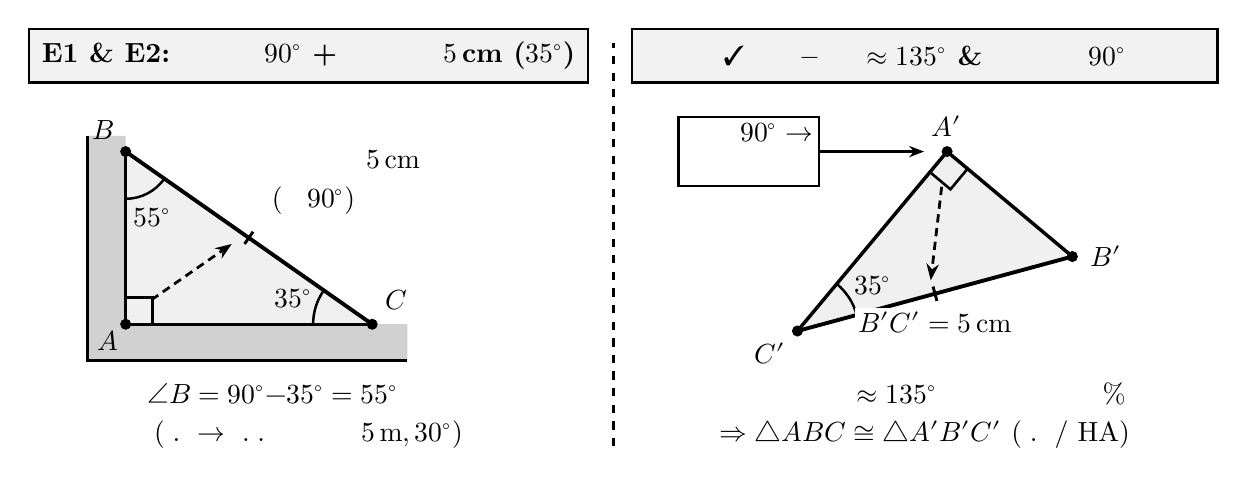
\begin{tikzpicture}[x=0.86cm, y=0.86cm, every node/.style={font=\fontsize{10pt}{13.8pt}\selectfont, text=black}]
  % --- ផ្នែកឆ្វេង៖ ផ្ទាំងកែង 90° + អ៊ីប៉ូតេនុស 5 cm មុំ 35° (x: 0.0..8.35) ---
  \begin{scope}[shift={(0.0, 0.0)}]
    \node[draw=black, fill=headgray, line width=0.95pt, minimum width=7.10cm, minimum height=0.68cm, anchor=south, font=\fontsize{10pt}{13.8pt}\selectfont] at (4.12, 4.45) {\textbf{\en{E1 \& E2:} ផ្ទាំងកែង $90^\circ$ \en{+} អ៊ីប៉ូតេនុស $5\unit{cm}$ ($35^\circ$)}};
    % ផ្ទាំងកែង 90° ខ្នាត 1:1 ពីក្រោយ
    \coordinate (A) at (1.42, 0.90);
    \coordinate (B) at (1.42, 3.45);
    \coordinate (C) at (5.06, 0.90);
    \fill[midgray] (0.86, 3.68) -- (0.86, 0.36) -- (5.58, 0.36) -- (5.58, 0.90) -- (1.42, 0.90) -- (1.42, 3.68) -- cycle;
    \draw[black, line width=0.95pt] (0.86, 3.68) -- (0.86, 0.36) -- (5.58, 0.36);
    \fill[panelgray] (A) -- (B) -- (C) -- cycle;
    \draw[black, line width=1.25pt] (B) -- (A) -- (C);
    \draw[black, line width=1.40pt, tk1] (B) -- (C);
    \pic[draw=black, line width=0.95pt, angle radius=3.4mm]{right angle=C--A--B};
    \pic[draw=black, line width=0.9pt, angle radius=7.5mm]{angle=B--C--A};
    \pic[draw=black, line width=0.9pt, angle radius=6.0mm]{angle=A--B--C};
    \node at ($(C)+(162:1.22)$) {$35^\circ$};
    \node at ($(B)+(-68:1.05)$) {$55^\circ$};
    % ព្រួញឈម 90° ទៅអ៊ីប៉ូតេនុស BC (ទុកគម្លាតស្អាត មិនប៉ះស្លាក)
    \draw[hypArrow] ($(A)+(0.38, 0.36)$) -- ($(B)!0.48!(C)+(-0.18, -0.14)$);
    \node[above right=2pt, align=left, fill=white, inner sep=1.5pt] at (3.45, 2.40) {អ៊ីប៉ូតេនុស $5\unit{cm}$\\(ឈម $90^\circ$)};
    \fill[black] (A) circle (2.0pt);
    \node at ($(A)+(-0.26, -0.24)$) {$A$};
    \fill[black] (B) circle (2.0pt) node[above left=1pt] {$B$};
    \fill[black] (C) circle (2.0pt) node[above right=2pt] {$C$};
    \node[align=center] at (4.12, -0.45) {មុំបំពេញ $\ang{B}=90^\circ{-}35^\circ=55^\circ$ ចាក់សោជ្រុងទាំង ៣\\(អ.ម $\to$ ម.ជ.ម និងជណ្ដើរ $5\unit{m}, 30^\circ$)};
  \end{scope}

  % បន្ទាត់បំបែកកណ្ដាល
  \draw[black, dashed, line width=0.95pt] (8.62, -0.90) -- (8.62, 5.05);

  % --- ផ្នែកស្ដាំ៖ ត្រីកោណកែងបង្វិល-ឆ្លុះ ~135° (x: 8.90..17.65) ---
  \begin{scope}[shift={(8.90, 0.0)}]
    \node[draw=black, fill=headgray, line width=0.95pt, minimum width=7.44cm, minimum height=0.68cm, anchor=south, font=\fontsize{10pt}{13.8pt}\selectfont] at (4.32, 4.45) {\textbf{\ding{51}\ បង្វិល\en{--}ឆ្លុះ $\approx 135^\circ$ \en{\&} ព្រួញប្រអប់ $90^\circ$}};
    \coordinate (Ap) at (4.65, 3.45);
    \coordinate (Bp) at (6.50, 1.90);
    \coordinate (Cp) at (2.44, 0.80);
    \fill[panelgray] (Ap) -- (Bp) -- (Cp) -- cycle;
    \draw[black, line width=1.25pt] (Cp) -- (Ap) -- (Bp);
    \draw[black, line width=1.40pt, tk1] (Bp) -- (Cp);
    \pic[draw=black, line width=0.95pt, angle radius=3.4mm]{right angle=Cp--Ap--Bp};
    \pic[draw=black, line width=0.9pt, angle radius=7.8mm]{angle=Bp--Cp--Ap};
    \node at ($(Cp)+(31:1.30)$) {$35^\circ$};
    % ព្រួញឈម 90° ពី A' ទៅ B'C'
    \draw[hypArrow] ($(Ap)+(-0.08, -0.52)$) -- ($(Bp)!0.52!(Cp)+(0.02, 0.22)$);
    \node[draw=black, fill=white, line width=0.8pt, inner sep=2.2pt, align=center] (arlbl) at (1.72, 3.45) {ប្រអប់ $90^\circ \to$\\ព្រួញអ៊ីប៉ូតេនុស};
    \draw[black, line width=0.85pt, -{Stealth[length=1.9mm]}] (arlbl.east) -- ($(Ap)+(-0.34, 0.00)$);
    \node[below=5pt, fill=white, inner sep=1.2pt] at ($(Bp)!0.50!(Cp)$) {$B'C' = 5\unit{cm}$};
    \fill[black] (Ap) circle (2.0pt) node[above=2pt] {$A'$};
    \fill[black] (Bp) circle (2.0pt) node[right=3pt] {$B'$};
    \fill[black] (Cp) circle (2.0pt) node[below left=1pt] {$C'$};
    \node[align=center] at (4.32, -0.45) {ត្រីកោណកែងបង្វិល $\approx 135^\circ$ នៅតែត្រួតស៊ីគ្នា ១០០\%\\$\Rightarrow \tri{ABC}\cg\tri{A'B'C'}$ (អ.ម / \en{HA})};
  \end{scope}
\end{tikzpicture}}

% រូបទី ២ (ផ្នែក ៥)៖ អន្ទាក់ POE 2A (អ៊ីប៉ូតេនុស 5cm vs ជ្រុងកែង 5cm) & POE 2B (ចម្ងាយកែង vs ទ្រេត)
\newcommand{\figGuidelineDualPOETraps}{%
\linespread{1.0}\selectfont
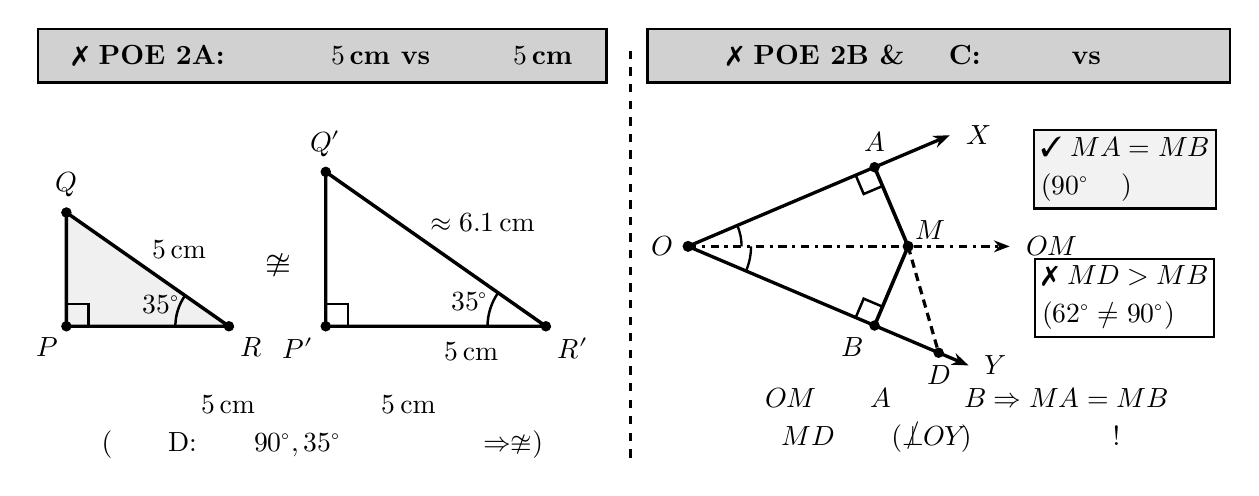
\begin{tikzpicture}[x=0.86cm, y=0.86cm, every node/.style={font=\fontsize{10pt}{13.8pt}\selectfont, text=black}]
  % --- ផ្នែកឆ្វេង៖ POE 2A អ៊ីប៉ូតេនុស 5cm vs ជ្រុងកែង 5cm (x: 0.0..8.50) ---
  \begin{scope}[shift={(0.0, 0.0)}]
    \node[draw=black, fill=midgray, line width=0.95pt, minimum width=7.22cm, minimum height=0.68cm, anchor=south, font=\fontsize{10pt}{13.8pt}\selectfont] at (4.20, 4.48) {\textbf{\ding{55}\ \en{POE 2A:} អ៊ីប៉ូតេនុស $5\unit{cm}$ \en{vs} ជ្រុងកែង $5\unit{cm}$}};
    % ត្រីកោណ PQR (អ៊ីប៉ូតេនុស 5cm)
    \coordinate (P) at (0.42, 0.90);
    \coordinate (R) at (2.82, 0.90);
    \coordinate (Q) at (0.42, 2.58);
    \fill[panelgray] (P) -- (Q) -- (R) -- cycle;
    \draw[black, line width=1.25pt] (P) -- (Q) -- (R) -- cycle;
    \pic[draw=black, line width=0.9pt, angle radius=2.8mm]{right angle=R--P--Q};
    \pic[draw=black, line width=0.9pt, angle radius=6.8mm]{angle=Q--R--P};
    \node at ($(R)+(162:1.05)$) {$35^\circ$};
    \node[above right=2pt, fill=white, inner sep=1.2pt] at ($(Q)!0.48!(R)$) {$5\unit{cm}$};
    \fill[black] (P) circle (1.9pt) node[below left=1pt] {$P$};
    \fill[black] (Q) circle (1.9pt) node[above=2pt] {$Q$};
    \fill[black] (R) circle (1.9pt) node[below right=1pt] {$R$};

    \node[font=\fontsize{12pt}{14pt}\selectfont] at (3.55, 1.80) {$\ncg$};

    % ត្រីកោណ P'Q'R' (ជ្រុងកែង P'R' = 5cm -> អ៊ីប៉ូតេនុស ≈ 6.1cm)
    \coordinate (Pp) at (4.25, 0.90);
    \coordinate (Rp) at (7.50, 0.90);
    \coordinate (Qp) at (4.25, 3.18);
    \fill[white] (Pp) -- (Qp) -- (Rp) -- cycle;
    \draw[black, line width=1.25pt] (Pp) -- (Qp) -- (Rp) -- cycle;
    \pic[draw=black, line width=0.9pt, angle radius=2.8mm]{right angle=Rp--Pp--Qp};
    \pic[draw=black, line width=0.9pt, angle radius=7.4mm]{angle=Qp--Rp--Pp};
    \node at ($(Rp)+(162:1.18)$) {$35^\circ$};
    \node[above right=2pt, fill=white, inner sep=1.2pt] at ($(Qp)!0.44!(Rp)$) {$\approx 6.1\unit{cm}$};
    \node[below=2pt] at ($(Pp)!0.50!(Rp)$) {ជ្រុងកែង $5\unit{cm}$};
    \fill[black] (Pp) circle (1.9pt) node[below left=1pt] {$P'$};
    \fill[black] (Qp) circle (1.9pt) node[above=2pt] {$Q'$};
    \fill[black] (Rp) circle (1.9pt) node[below right=1pt] {$R'$};

    \node[align=center] at (4.20, -0.58) {ប្រើជ្រុងកែង $5\unit{cm}$ ទល់អ៊ីប៉ូតេនុស $5\unit{cm}$ មិនប៉ុនគ្នាទេ\\(និងកាត \en{D:} មានតែ $90^\circ, 35^\circ$ គ្មានអ៊ីប៉ូតេនុស $\Rightarrow \ncg$)};
  \end{scope}

  % បន្ទាត់បំបែកកណ្ដាល
  \draw[black, dashed, line width=0.95pt] (8.75, -1.04) -- (8.75, 5.08);

  % --- ផ្នែកស្ដាំ៖ POE 2B ចម្ងាយកែង MA=MB vs ទ្រេត MD (x: 9.00..17.65) ---
  \begin{scope}[shift={(9.00, 0.0)}]
    \node[draw=black, fill=midgray, line width=0.95pt, minimum width=7.40cm, minimum height=0.68cm, anchor=south, font=\fontsize{10pt}{13.8pt}\selectfont] at (4.30, 4.48) {\textbf{\ding{55}\ \en{POE 2B \&} កាត \en{C:} ចម្ងាយកែង \en{vs} ទ្រេត}};
    \coordinate (O) at (0.60, 2.08);
    \coordinate (X) at ($(O)+(23:4.20)$);
    \coordinate (Y) at ($(O)+(-23:4.50)$);
    \coordinate (M) at ($(O)+(0:3.25)$);
    \coordinate (Mend) at ($(O)+(0:4.75)$);
    \coordinate (A) at ($(O)+(23:2.992)$);
    \coordinate (B) at ($(O)+(-23:2.992)$);
    \coordinate (D) at ($(O)+(-23:4.02)$);

    \draw[black, line width=1.2pt, -{Stealth[length=2.1mm]}] (O) -- (X) node[right=2pt] {$X$};
    \draw[black, line width=1.2pt, -{Stealth[length=2.1mm]}] (O) -- (Y) node[right=2pt] {$Y$};
    \draw[black, line width=1.15pt, dash dot, -{Stealth[length=2.0mm]}] (O) -- (Mend) node[right=2pt] {$OM$};

    \draw[black, line width=1.30pt] (M) -- (A);
    \draw[black, line width=1.30pt] (M) -- (B);
    \draw[black, line width=1.15pt, densely dashed] (M) -- (D);

    \pic[draw=black, line width=0.9pt, angle radius=2.6mm]{right angle=O--A--M};
    \pic[draw=black, line width=0.9pt, angle radius=2.6mm]{right angle=O--B--M};
    \pic[draw=black, line width=0.85pt, angle radius=6.8mm]{angle=M--O--X};
    \pic[draw=black, line width=0.85pt, angle radius=8.0mm]{angle=Y--O--M};

    \fill[black] (O) circle (2.0pt) node[left=2pt] {$O$};
    \fill[black] (M) circle (2.0pt) node[above right=2pt, fill=white, inner sep=1pt] {$M$};
    \fill[black] (A) circle (1.9pt) node[above=2pt] {$A$};
    \fill[black] (B) circle (1.9pt) node[below left=1pt] {$B$};
    \fill[black] (D) circle (1.9pt) node[below=1pt] {$D$};

    \node[draw=black, fill=headgray, line width=0.8pt, inner sep=2.5pt, align=left] at (7.05, 3.22) {\ding{51}\ $MA=MB$\\($90^\circ$ កែង)};
    \node[draw=black, fill=white, line width=0.8pt, inner sep=2.5pt, align=left] at (7.05, 1.32) {\ding{55}\ $MD > MB$\\($62^\circ \neq 90^\circ$)};

    \node[align=center] at (4.30, -0.48) {បត់តាម $OM$ ផ្ទៀង $A$ ត្រួតលើ $B \Rightarrow MA=MB$\\តែ $MD$ ទ្រេត ($\not\perp OY$) មិនមែនចម្ងាយកែងទេ!};
  \end{scope}
\end{tikzpicture}}

% រូបទី ៣ (ផ្នែក ៥)៖ កែកំហុសសៀវភៅគោលទំព័រ ១៥៣ (1a, 1b & 1c គ្មាន / លើ OA, OB)
\newcommand{\figGuidelineErrataAndModel}{%
\linespread{1.0}\selectfont
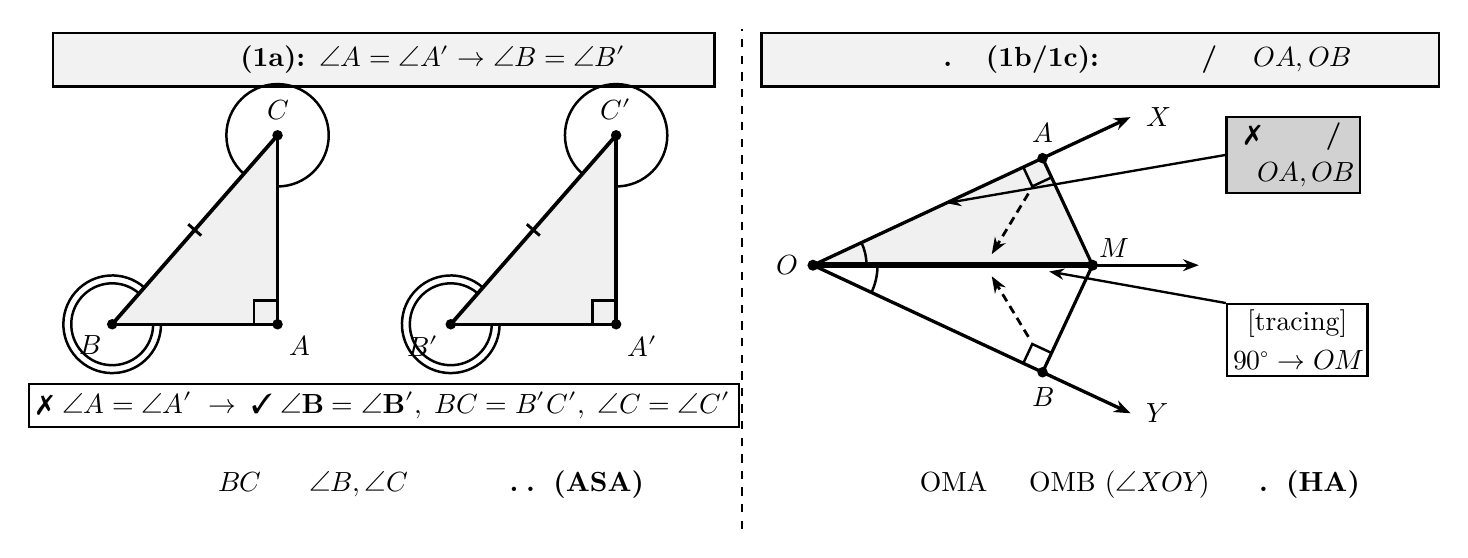
\begin{tikzpicture}[x=1cm, y=1cm, every node/.style={font=\fontsize{10pt}{13.8pt}\selectfont, text=black}]
  % --- ផ្នែកឆ្វេង៖ កែ 1a សម្រាយទំព័រ 153 (∠A=∠A' -> ∠B=∠B') (x: 0.0..8.50) ---
  \begin{scope}[shift={(0.0, 0.0)}]
    \node[draw=black, fill=headgray, line width=0.95pt, minimum width=8.40cm, minimum height=0.68cm, anchor=south, font=\fontsize{10pt}{13.8pt}\selectfont] at (4.20, 4.45) {\textbf{កែទំព័រ ១៥៣ (\en{1a}): $\ang{A}=\ang{A'}\to\ang{B}=\ang{B'}$}};
    % ∆ABC តាមទម្រង់សៀវភៅទំ.១៥៣
    \coordinate (A) at (2.85, 1.45);
    \coordinate (B) at (0.75, 1.45);
    \coordinate (C) at (2.85, 3.85);
    \fill[panelgray] (A) -- (B) -- (C) -- cycle;
    \draw[black, line width=1.25pt] (B) -- (A) -- (C);
    \draw[black, line width=1.35pt, tk1] (B) -- (C);
    \pic[draw=black, line width=0.9pt, angle radius=3.0mm]{right angle=C--A--B};
    \pic[draw=black, line width=0.9pt, angle radius=6.5mm]{angle=A--C--B};
    \pic[draw=black, line width=0.9pt, angle radius=5.2mm]{angle=C--B--A};
    \pic[draw=black, line width=0.9pt, angle radius=6.2mm]{angle=C--B--A};
    \fill[black] (A) circle (1.9pt) node[below right=1pt] {$A$};
    \fill[black] (B) circle (1.9pt) node[below left=1pt] {$B$};
    \fill[black] (C) circle (1.9pt) node[above=2pt] {$C$};

    % ∆A'B'C'
    \coordinate (Ap) at (7.15, 1.45);
    \coordinate (Bp) at (5.05, 1.45);
    \coordinate (Cp) at (7.15, 3.85);
    \fill[panelgray] (Ap) -- (Bp) -- (Cp) -- cycle;
    \draw[black, line width=1.25pt] (Bp) -- (Ap) -- (Cp);
    \draw[black, line width=1.35pt, tk1] (Bp) -- (Cp);
    \pic[draw=black, line width=0.9pt, angle radius=3.0mm]{right angle=Cp--Ap--Bp};
    \pic[draw=black, line width=0.9pt, angle radius=6.5mm]{angle=Ap--Cp--Bp};
    \pic[draw=black, line width=0.9pt, angle radius=5.2mm]{angle=Cp--Bp--Ap};
    \pic[draw=black, line width=0.9pt, angle radius=6.2mm]{angle=Cp--Bp--Ap};
    \fill[black] (Ap) circle (1.9pt) node[below right=1pt] {$A'$};
    \fill[black] (Bp) circle (1.9pt) node[below left=1pt] {$B'$};
    \fill[black] (Cp) circle (1.9pt) node[above=2pt] {$C'$};

    \node[draw=black, fill=white, line width=0.85pt, inner sep=3pt] at (4.20, 0.42) {\ding{55}\ $\ang{A}=\ang{A'}\;\to\;\mathbf{\text{\ding{51}}\;\ang{B}=\ang{B'}},\; BC=B'C',\; \ang{C}=\ang{C'}$};
    \node[align=center] at (4.20, -0.58) {អ៊ីប៉ូតេនុស $BC$ ជាប់ $\ang{B}, \ang{C}$ ទើបសរុបតាម \textbf{ម.ជ.ម (\en{ASA})}};
  \end{scope}

  % បន្ទាត់បំបែកកណ្ដាល
  \draw[black, dashed, line width=0.95pt] (8.75, -1.15) -- (8.75, 5.20);

  % --- ផ្នែកស្ដាំ៖ លំហាត់គំរូទំ.១៥៣ (1b/1c) គ្មាន / លើ OA, OB (x: 9.00..17.65) ---
  \begin{scope}[shift={(9.00, 0.0)}]
    \node[draw=black, fill=headgray, line width=0.95pt, minimum width=8.60cm, minimum height=0.68cm, anchor=south, font=\fontsize{10pt}{13.8pt}\selectfont] at (4.30, 4.45) {\textbf{លំហាត់គំរូទំ.១៥៣ (\en{1b/1c}): គ្មានគំនូស \en{/} លើ $OA, OB$}};
    \coordinate (O) at (0.65, 2.20);
    \coordinate (X) at ($(O)+(25:4.45)$);
    \coordinate (Y) at ($(O)+(-25:4.45)$);
    \coordinate (M) at ($(O)+(0:3.55)$);
    \coordinate (Mend) at ($(O)+(0:4.90)$);
    \coordinate (A) at ($(O)+(25:3.217)$);
    \coordinate (B) at ($(O)+(-25:3.217)$);

    \fill[panelgray] (O) -- (A) -- (M) -- cycle;
    \fill[white] (O) -- (B) -- (M) -- cycle;
    \draw[black, line width=1.2pt, -{Stealth[length=2.1mm]}] (O) -- (X) node[right=2pt] {$X$};
    \draw[black, line width=1.2pt, -{Stealth[length=2.1mm]}] (O) -- (Y) node[right=2pt] {$Y$};
    \draw[black, line width=1.15pt] (A) -- (M) -- (B);
    % អ៊ីប៉ូតេនុសរួម OM ដិតច្បាស់ (គ្មានគំនូស / លើ OA, OB ដាច់ខាត!)
    \draw[black, line width=2.3pt] (O) -- (M);
    \draw[black, line width=1.1pt, -{Stealth[length=2.0mm]}] (M) -- (Mend);

    \pic[draw=black, line width=0.9pt, angle radius=2.7mm]{right angle=O--A--M};
    \pic[draw=black, line width=0.9pt, angle radius=2.7mm]{right angle=O--B--M};
    \pic[draw=black, line width=0.9pt, angle radius=6.8mm]{angle=M--O--X};
    \pic[draw=black, line width=0.9pt, angle radius=8.2mm]{angle=Y--O--M};

    % ព្រួញ [tracing] ពី 90° ទៅ OM
    \draw[hypArrow] ($(A)+(-0.18,-0.45)$) -- (2.92, 2.34);
    \draw[hypArrow] ($(B)+(-0.18,0.45)$) -- (2.92, 2.06);

    \fill[black] (O) circle (2.0pt) node[left=2pt] {$O$};
    \fill[black] (A) circle (1.9pt) node[above=2pt] {$A$};
    \fill[black] (B) circle (1.9pt) node[below=2pt] {$B$};
    \fill[black] (M) circle (2.0pt) node[above right=2pt, fill=white, inner sep=1pt] {$M$};

    \node[draw=black, fill=midgray, line width=0.8pt, inner sep=2.2pt, align=center] (notick) at (6.75, 3.60) {\ding{55}\ ហាមគូស \textbf{/}\\លើ $OA, OB$};
    \draw[black, line width=0.85pt, -{Stealth[length=1.9mm]}] (notick.west) -- ($(O)!0.58!(A)$);
    \node[draw=black, fill=white, line width=0.8pt, inner sep=2.2pt, align=center] (trbox) at (6.80, 1.25) {\en{[tracing]}\\$90^\circ \to OM$};
    \draw[black, line width=0.85pt, -{Stealth[length=1.9mm]}] (trbox.north west) -- (3.65, 2.12);

    \node[align=center] at (4.30, -0.58) {កែអត្ថបទ៖ \en{OMA} និង \en{OMB} ($\ang{XOY}$) តាម \textbf{អ.ម (\en{HA})}};
  \end{scope}
\end{tikzpicture}}

% រូបទី ៤ (ផ្នែក ៥)៖ ប្រតិបត្តិទំព័រ ១៥៤ បំបែកត្រីកោណត្រួតគ្នា & កិច្ចការផ្ទះ #6 vs #7
\newcommand{\figGuidelinePracticeAndHW}{%
\linespread{1.0}\selectfont
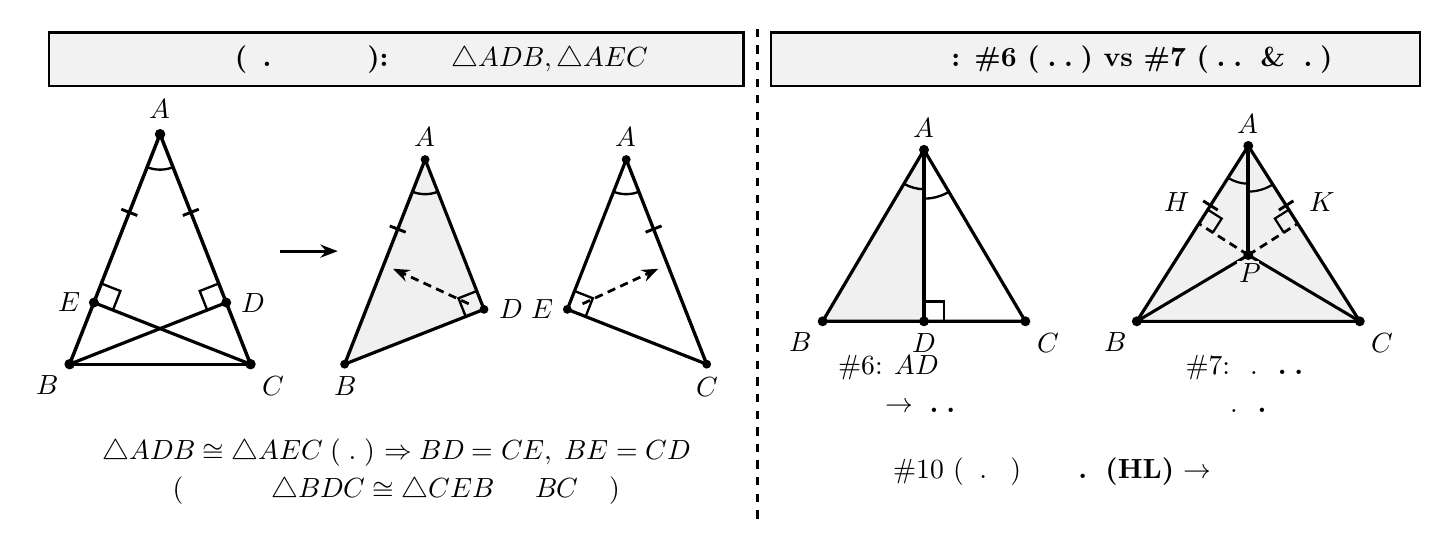
\begin{tikzpicture}[x=0.99cm, y=0.99cm, every node/.style={font=\fontsize{10pt}{13.8pt}\selectfont, text=black}]
  % --- ផ្នែកឆ្វេង៖ ប្រតិបត្តិទំព័រ ១៥៤ (x: 0.0..8.82) ---
  \begin{scope}[shift={(0.0, 0.0)}]
    \node[draw=black, fill=headgray, line width=0.95pt, minimum width=8.82cm, minimum height=0.68cm, anchor=south, font=\fontsize{10pt}{13.8pt}\selectfont] at (4.41, 4.45) {\textbf{ប្រតិបត្តិ (ទំ.១៥៤ គ្មានរូប): បំបែក $\tri{ADB}, \tri{AEC}$}};
    % រូបគោល ∆ABC
    \coordinate (A) at (1.38, 3.85);
    \coordinate (B) at (0.22, 0.90);
    \coordinate (C) at (2.54, 0.90);
    \coordinate (D) at ($(A)!(B)!(C)$);
    \coordinate (E) at ($(A)!(C)!(B)$);
    \draw[black, line width=1.25pt, tk1low] (A) -- (B);
    \draw[black, line width=1.25pt, tk1low] (A) -- (C);
    \draw[black, line width=1.20pt] (B) -- (C);
    \draw[black, line width=1.15pt] (B) -- (D);
    \draw[black, line width=1.15pt] (C) -- (E);
    \pic[draw=black, line width=0.85pt, angle radius=2.6mm]{right angle=A--D--B};
    \pic[draw=black, line width=0.85pt, angle radius=2.6mm]{right angle=A--E--C};
    \pic[draw=black, line width=0.85pt, angle radius=4.5mm]{angle=B--A--C};
    \fill[black] (A) circle (1.9pt) node[above=2pt] {$A$};
    \fill[black] (B) circle (1.9pt) node[below left=1pt] {$B$};
    \fill[black] (C) circle (1.9pt) node[below right=1pt] {$C$};
    \fill[black] (D) circle (1.8pt) node[right=2pt] {$D$};
    \fill[black] (E) circle (1.8pt) node[left=2pt] {$E$};

    % ព្រួញបំបែក
    \draw[black, line width=1.15pt, -{Stealth[length=2.2mm]}] (2.92, 2.35) -- (3.66, 2.35);
    \node[above=2pt] at (3.29, 2.38) {បំបែក};

    % បំបែក ∆ADB
    \begin{scope}[shift={(4.78, 0.90)}, scale=0.89]
      \coordinate (A1) at (0, 2.95); \coordinate (B1) at (-1.16, 0); \coordinate (C1) at (1.16, 0);
      \coordinate (D1) at ($(A1)!(B1)!(C1)$);
      \fill[panelgray] (A1) -- (B1) -- (D1) -- cycle;
      \draw[black, line width=1.20pt, tk1low] (A1) -- (B1);
      \draw[black, line width=1.15pt] (A1) -- (D1) -- (B1);
      \pic[draw=black, line width=0.85pt, angle radius=2.5mm]{right angle=A1--D1--B1};
      \pic[draw=black, line width=0.85pt, angle radius=4.4mm]{angle=B1--A1--D1};
      \draw[hypArrow] ($(D1)+(-0.22, 0.08)$) -- ($(A1)!0.52!(B1)+(0.14,-0.04)$);
      \fill[black] (A1) circle (1.8pt) node[above=1pt] {$A$};
      \fill[black] (B1) circle (1.8pt) node[below=1pt] {$B$};
      \fill[black] (D1) circle (1.8pt) node[right=2pt] {$D$};
    \end{scope}

    % បំបែក ∆AEC
    \begin{scope}[shift={(7.36, 0.90)}, scale=0.89]
      \coordinate (A2) at (0, 2.95); \coordinate (B2) at (-1.16, 0); \coordinate (C2) at (1.16, 0);
      \coordinate (E2) at ($(A2)!(C2)!(B2)$);
      \fill[white] (A2) -- (C2) -- (E2) -- cycle;
      \draw[black, line width=1.20pt, tk1low] (A2) -- (C2);
      \draw[black, line width=1.15pt] (A2) -- (E2) -- (C2);
      \pic[draw=black, line width=0.85pt, angle radius=2.5mm]{right angle=A2--E2--C2};
      \pic[draw=black, line width=0.85pt, angle radius=4.4mm]{angle=E2--A2--C2};
      \draw[hypArrow] ($(E2)+(0.22, 0.08)$) -- ($(A2)!0.52!(C2)+(-0.14,-0.04)$);
      \fill[black] (A2) circle (1.8pt) node[above=1pt] {$A$};
      \fill[black] (C2) circle (1.8pt) node[below=1pt] {$C$};
      \fill[black] (E2) circle (1.8pt) node[left=2pt] {$E$};
    \end{scope}

    \node[align=center] at (4.41, -0.48) {$\tri{ADB}\cg\tri{AEC}$ (អ.ម) $\Rightarrow BD=CE,\; BE=CD$\\(ឬវិធីទី ២៖ $\tri{BDC}\cg\tri{CEB}$ តាម $BC$ រួម)};
  \end{scope}

  % បន្ទាត់បំបែកកណ្ដាល
  \draw[black, dashed, line width=0.95pt] (9.04, -1.08) -- (9.04, 5.20);

  % --- ផ្នែកស្ដាំ៖ កិច្ចការផ្ទះ #6 (ម.ជ.ម) vs #7 (ជ.ម.ជ & អ.ម) (x: 9.26..17.50) ---
  \begin{scope}[shift={(9.26, 0.0)}]
    \node[draw=black, fill=headgray, line width=0.95pt, minimum width=8.24cm, minimum height=0.68cm, anchor=south, font=\fontsize{10pt}{13.8pt}\selectfont] at (4.12, 4.45) {\textbf{កិច្ចការផ្ទះ: \en{\#6} (ម.ជ.ម) \en{vs \#7} (ជ.ម.ជ \en{\&} អ.ម)}};
    % លំហាត់ទី ៦
    \coordinate (A6) at (1.92, 3.65);
    \coordinate (B6) at (0.62, 1.45);
    \coordinate (C6) at (3.22, 1.45);
    \coordinate (D6) at (1.92, 1.45);
    \fill[panelgray] (A6) -- (B6) -- (D6) -- cycle;
    \draw[black, line width=1.15pt] (A6) -- (B6) -- (C6) -- cycle;
    \draw[black, line width=1.70pt] (A6) -- (D6);
    \pic[draw=black, line width=0.85pt, angle radius=2.5mm]{right angle=A6--D6--C6};
    \pic[draw=black, line width=0.85pt, angle radius=5.0mm]{angle=B6--A6--D6};
    \pic[draw=black, line width=0.85pt, angle radius=6.2mm]{angle=D6--A6--C6};
    \fill[black] (A6) circle (1.8pt) node[above=1pt] {$A$};
    \fill[black] (B6) circle (1.8pt) node[below left=1pt] {$B$};
    \fill[black] (C6) circle (1.8pt) node[below right=1pt] {$C$};
    \fill[black] (D6) circle (1.8pt) node[below=1pt] {$D$};
    \node[align=center] at (1.92, 0.65) {\en{\#6:} $AD$ ជ្រុងកែង\\$\to$ \textbf{ម.ជ.ម}};

    % លំហាត់ទី ៧
    \coordinate (A7) at (6.08, 3.70);
    \coordinate (B7) at (4.65, 1.45);
    \coordinate (C7) at (7.51, 1.45);
    \coordinate (P7) at (6.08, 2.30);
    \coordinate (H7) at ($(A7)!(P7)!(B7)$);
    \coordinate (K7) at ($(A7)!(P7)!(C7)$);
    \fill[panelgray] (A7) -- (B7) -- (C7) -- cycle;
    \draw[black, line width=1.15pt, tk1low] (A7) -- (B7);
    \draw[black, line width=1.15pt, tk1low] (A7) -- (C7);
    \draw[black, line width=1.10pt] (B7) -- (C7) (B7) -- (P7) -- (C7);
    \draw[black, line width=1.50pt] (A7) -- (P7);
    \draw[black, line width=1.00pt, densely dashed] (P7) -- (H7) (P7) -- (K7);
    \pic[draw=black, line width=0.8pt, angle radius=2.1mm]{right angle=A7--H7--P7};
    \pic[draw=black, line width=0.8pt, angle radius=2.1mm]{right angle=A7--K7--P7};
    \pic[draw=black, line width=0.8pt, angle radius=4.8mm]{angle=B7--A7--P7};
    \pic[draw=black, line width=0.8pt, angle radius=5.8mm]{angle=P7--A7--C7};
    \fill[black] (A7) circle (1.8pt) node[above=1pt] {$A$};
    \fill[black] (B7) circle (1.8pt) node[below left=1pt] {$B$};
    \fill[black] (C7) circle (1.8pt) node[below right=1pt] {$C$};
    \fill[black] (P7) circle (1.8pt) node[below=2pt, fill=panelgray, inner sep=0.8pt] {$P$};
    \node[above left=1pt] at (H7) {$H$};
    \node[above right=1pt] at (K7) {$K$};
    \node[align=center] at (6.08, 0.65) {\en{\#7:} ក. \textbf{ជ.ម.ជ}\\ខ. \textbf{អ.ម}};

    \node[align=center] at (4.12, -0.48) {រីឯ \en{\#10} (ទំ.១៦៥) ប្រើ \textbf{អ.ជ (\en{HL})} $\to$ លើកទៅចំណិតទី ៣};
  \end{scope}
\end{tikzpicture}}

% ============================================================================
% ចាប់ផ្ដើមឯកសារ (Document Body)
% ============================================================================
\begin{document}
\thispagestyle{firstpage}
\fontsize{11.5pt}{14.92pt}\selectfont
\vspace*{-0.75cm}

% -------------------- ក្បាលរដ្ឋបាលផ្លូវការ (Verbatim Match to LS_Plan_HA.tex) --------------------
\begin{center}
  {\muol\fontsize{13pt}{18pt}\selectfont ព្រះរាជាណាចក្រកម្ពុជា}\\[2pt]
  {\muol\fontsize{12pt}{17pt}\selectfont ជាតិ សាសនា ព្រះមហាក្សត្រ}\\[1pt]
  \khmflourish
\end{center}

\vspace{-12pt}
{\muol\fontsize{10.8pt}{15.5pt}\selectfont
មន្ទីរអប់រំ យុវជន និងកីឡា ខេត្តកំពង់ធំ\\
ការិយាល័យអប់រំ យុវជន និងកីឡា ស្រុកកំពង់ស្វាយ\\
អនុវិទ្យាល័យព្រះក្រសាំង}

\vspace{6pt}
\begin{center}
  \parttitle{មគ្គុទ្ទេសក៍គរុកោសល្យគ្រូ និងរបាយការណ៍ស្រាវជ្រាវសង្ខេប}\\[3pt]
  {\muol\fontsize{11.5pt}{16.5pt}\selectfont ករណីត្រីកោណកែងប៉ុនគ្នា៖ អ\enbf{.}ម \enbf{(HA)} និងលក្ខណៈពុះមុំ}
\end{center}

\vspace{4pt}

% ============================================================================
% ប្រអប់ព័ត៌មានទូទៅនៃមេរៀន និងកញ្ចប់ឯកសារភ្ជាប់
% ============================================================================
\begin{tcolorbox}[
  enhanced, sharp corners, breakable, colback=panelgray, colframe=black,
  colbacktitle=black!12, coltitle=black, titlerule=0.7pt,
  fonttitle=\fontsize{11pt}{14.5pt}\selectfont,
  fontupper=\fontsize{11.5pt}{14.92pt}\selectfont,
  title={\muol\fontsize{11pt}{14.5pt}\selectfont ព័ត៌មានទូទៅនៃមេរៀន និងកញ្ចប់ឯកសារភ្ជាប់ \enbf{(Grade 8 HA)}},
  boxrule=1.0pt, top=6pt, bottom=6pt, left=6pt, right=6pt,
  toptitle=4pt, bottomtitle=4pt, before skip=4pt, after skip=8pt
]
  \linespread{1.0}\selectfont
  \renewcommand{\arraystretch}{1.22}
  \setlength{\tabcolsep}{0.9pt}
  \begin{tabular}{@{}L{3.08cm} L{0.15cm} L{5.76cm} L{2.36cm} L{0.15cm} L{5.35cm}@{}}
    - មុខវិជ្ជា & : & គណិតវិទ្យា ថ្នាក់ទី៨ & - រយៈពេល & : & ១ ម៉ោងសិក្សា (៥០ នាទី) \\
    - ចំណងជើងមេរៀន & : & មេរៀនទី១២ ការប្រៀបធៀបត្រីកោណ & - បង្រៀនដោយ & : & ហុក ប៊ុនថែន \\
    - ចំណងជើងរង & : & ១.៣.១ ករណី អ.ម \textbf{(HA)} \& ពុះមុំ & - កាលបរិច្ឆេទ & : & ថ្ងៃសៅរ៍ ទី២៨ ខែវិច្ឆិកា ឆ្នាំ២០២៦ \\
  \end{tabular}\\[4pt]
  \fontsize{11.5pt}{14.92pt}\selectfont\linespread{1.22}\selectfont
  \textbf{ឯកសារភ្ជាប់ក្នុងកញ្ចប់បង្រៀន (\en{NGS 5Es Lesson Package})៖}
  (១) \en{LS\_\allowbreak Plan\_\allowbreak HA.pdf} (កិច្ចតែងការបង្រៀន \en{5Es} ៥០ នាទី),
  (២) \en{Teaching\_\allowbreak Scenario\_\allowbreak HA.pdf} (សេណារីយ៉ូបង្រៀន ៥០ នាទី),
  (៣) \en{Printable\_\allowbreak Materials\_\allowbreak HA.pdf} (សម្ភារៈបោះពុម្ព ស-ខ្មៅ ខ្នាតពិត \en{1:1} ចំនួន ៦ ទំព័រ),
  (៤) \en{Teaching\_\allowbreak Guideline\_\allowbreak HA.pdf} (មគ្គុទ្ទេសក៍គរុកោសល្យគ្រូនេះ),
  និង (៥) ថតភស្តុតាង ឯកសារ\allowbreak ស្រាវជ្រាវ\allowbreak យោង\_\allowbreak\en{PDF/} (\en{Open-Access PDFs} + \en{Evidence Index})។
\end{tcolorbox}

% ============================================================================
% ផ្នែកទី ១៖ បរិបទមេរៀន និងទិដ្ឋភាពទូទៅគរុកោសល្យ
% ============================================================================
\secbanner{ផ្នែកទី ១៖ បរិបទមេរៀន និងទិដ្ឋភាពទូទៅគរុកោសល្យ}{Section 1: Administrative Context, Grade 8 Kampong Svay Setting \& 50-Min Overview}

\subsec{១\enbf{.}១ បរិបទថ្នាក់ទី៨ អនុវិទ្យាល័យព្រះក្រសាំង និងតម្រូវការបង្រៀនករណី អ\enbf{.}ម \enbf{(HA)}}

នៅអនុវិទ្យាល័យព្រះក្រសាំង (ស្រុកកំពង់ស្វាយ ខេត្តកំពង់ធំ) ក្រោយពីសិស្សថ្នាក់ទី៨ បានរៀនចប់ករណីទូទៅទាំងបីគឺ ម.ជ.ម (\en{ASA}), ជ.ម.ជ (\en{SAS}), និង ជ.ជ.ជ (\en{SSS}) រួចហើយ សិស្សឈានចូល \textbf{§១.៣.១ ករណីត្រីកោណកែង៖ អ៊ីប៉ូតេនុសប៉ុនគ្នា និងមុំស្រួចមួយប៉ុនគ្នា (អ.ម / \en{HA}) និងលក្ខណៈពុះមុំ} ក្នុងសៀវភៅសិក្សាគោលថ្នាក់ទី៨ ទំព័រ \textbf{១៥៣--១៥៤} (ព្រមទាំងលំហាត់ទី៦ ទំព័រ \textbf{១៦៤} និងលំហាត់ទី៧ ទំព័រ \textbf{១៦៥})។ បើគ្រូបង្រៀនតាមទម្លាប់ចាស់ដោយសរសេរនិយមន័យត្រង់ៗលើក្ដារខៀន សិស្សនឹងជួបបញ្ហាធ្ងន់ធ្ងរ ៥ យ៉ាង៖
\begin{itemize}[leftmargin=0.55cm, topsep=1pt, itemsep=1.5pt, parsep=0pt]
  \item \textbf{១) ការភ័ន្តច្រឡំរវាងអ៊ីប៉ូតេនុស ជ្រុងកែង និងទិសដៅបង្វិល៖} សិស្សមិនស្គាល់ច្បាស់ថាអ៊ីប៉ូតេនុសស្ថិតនៅឈមមុំ $90^\circ$ ហើយតែងច្រឡំករណី អ.ម (\en{HA}) ជាមួយជ្រុងជាប់កែង (\en{LA}) ឬមុំដូចគ្នា (\en{AA}) ជាពិសេសពេលត្រីកោណកែងបង្វិល $\approx 135^\circ$ \en{(Bilik Durmaz \& Isiksal Bostan, 2022; Ubah \& Bansilal, 2019; Yigit Koyunkaya, 2018)}។
  \item \textbf{២) កំហុសចម្ងាយទ្រេត និងការបត់កន្លះបន្ទាត់ពុះមុំ៖} សិស្សងាយជឿថាបន្ទាត់កែងត្រូវតែឈរត្រង់ (គំនូរគំរូ) ហើយវាស់ចម្ងាយពីចំណុច $M$ ទៅជ្រុងមុំតាមអង្កត់ទ្រេតមិនកែង $MD$ ព្រមទាំងច្រឡំទ្រឹស្ដីបទពុះមុំផ្ទាល់ និងច្រាស \en{(Catman-Aksoy \& Isiksal-Bostan, 2024; Boz-Yaman, 2024; Šipuš et al., 2022)}។
  \item \textbf{៣) កំហុសបោះពុម្ពសៀវភៅគោលទំព័រ ១៥៣ (\en{Errata 1a, 1b} \& \en{Trap 1c})៖} សៀវភៅគោលទំព័រ ១៥៣ បោះពុម្ពភ័ន្តដង្កៀប \en{ASA} ជា $\ang{A}=\ang{A'}=90^\circ$ ជំនួសឱ្យ \textbf{$\ang{B}=\ang{B'}$}, បោះឈ្មោះលំហាត់គំរូជា «$OMA$ និង $OMA$» (និង $\ang{AOB}$) ជំនួសឱ្យ «\textbf{$OMA$ និង $OMB$}» ($\ang{XOY}$), និងគូសសញ្ញាស្មើគ្នា \tickone\ ទុកមុនលើ $OA, OB$ ដែលជំរុញឱ្យសិស្សបន្ថែមបម្រាប់មិនពិត \en{(Shahbari \& Daher, 2020)}។
  \item \textbf{៤) ប្រធាន «ប្រតិបត្តិ» ទំព័រ ១៥៤ គ្មានរូប និងត្រីកោណកែងត្រួតគ្នា៖} សិស្សថ្នាក់ទី៨ មានអត្រាទាបក្នុងការគូសកម្ពស់ត្រីកោណកែង ($8\%$ មុនរៀន) ហើយងាយធ្លាក់ចុះនៅពេលត្រីកោណត្រួតគ្នា និងពេលប្រធានគ្មានរូបភាពបង្ហាញ \en{(Yıldız et al., 2010; Biber, 2020; Winer \& Battista, 2022)}។
  \item \textbf{៥) ព្រំដែនជាមួយចំណិតទី ៣ (អ.ជ / \en{HL})៖} សៀវភៅទំព័រ ១៥៤ មិនទាន់ស្រាយទ្រឹស្ដីបទពុះមុំច្រាសទេ ហើយ\textbf{លំហាត់ទី១០ ទំព័រ ១៦៥} ត្រូវការលក្ខខណ្ឌអ៊ីប៉ូតេនុស និងជ្រុងកែងមួយ (អ.ជ / \en{HL}) ទើបត្រូវលើកទៅចំណិតទី ៣ (១.៣.២)។
\end{itemize}

\subsec{១\enbf{.}២ ដំណើរសាច់រឿង ៥០ នាទី \enbf{(2 + 9 + 17 + 20 + 2 min)} និងសមាហរណកម្មកញ្ចប់ឯកសារ ៤}

មេរៀនត្រូវបានរៀបចំតាមរយៈពេលស្តង់ដារ \textbf{៥០ នាទីពេញ} ក្រោមតួនាទី \textbf{«ក្រុមស្ថាបត្យករជណ្ដើរសុវត្ថិភាព»} (៣ នាក់/ក្រុម) សមកាលកម្ម ១០០\% រវាង \en{LS\_\allowbreak Plan\_\allowbreak HA.tex}, \en{Teaching\_\allowbreak Scenario\_\allowbreak HA.tex}, និង \en{Printable\_\allowbreak Materials\_\allowbreak HA.pdf} (ទំព័រ ១--៦)៖
\begin{itemize}[leftmargin=0.55cm, topsep=1pt, itemsep=1.5pt, parsep=0pt]
  \item \textbf{ជំហានទី ១ (00--02 \en{min} | ២ នាទី)៖} រដ្ឋបាលថ្នាក់ ចាត់ «ក្រុមស្ថាបត្យករជណ្ដើរសុវត្ថិភាព» ៣ នាក់/ក្រុម និងចែកកញ្ចប់សន្លឹក ១:១ (ទំព័រ ១) ទុកលើតុ។
  \item \textbf{ជំហានទី ២ (02--11 \en{min} | ៩ នាទី = ៣ + ៣ + ៣)៖} (ក) កំណែកិច្ចការផ្ទះ មេរៀន \en{SSS} (លំហាត់ \#4 ទំ.១៦៤ ខ្លែង $ABCD$ និង \#9 ទំ.១៦៥ $\tri{ABC}\cg\tri{DCB}$ + សំណួរបញ្ឆោត $\tri{ABC}\cg\tri{BDC}$); (ខ) រំលឹករហ័ស ២ ភាគ (អ៊ីប៉ូតេនុស $BC$ ឈម $90^\circ$ និង $\ang{B}=90^\circ{-}\ang{C}=55^\circ$; ចម្ងាយកែង $MA\perp OX$ vs ទ្រេត $MD$); (គ) \textbf{\en{E1 Engage}}៖ រឿង «ជម្រាលជណ្ដើរសុវត្ថិភាព $5\unit{m}$ ($30^\circ$) និងទ្វារទឹក $M$ លើពុះមុំប្រឡាយ $OX, OY$»។
  \item \textbf{ជំហានទី ៣ (11--28 \en{min} | ១៧ នាទី = ១១ + ៦)៖} \textbf{\en{E2 Explore (11 min)}}៖ សកម្មភាព ១ (៦ នាទី៖ ផ្ទាំងកែង $90^\circ$ + អ៊ីប៉ូតេនុស $5\unit{cm}$ មុំ $35^\circ$ កាត់ត្រួតបង្វិល-ឆ្លុះ $\sim 135^\circ$ ទំព័រ ១) និងសកម្មភាព ២ \en{Dual POE} (៥ នាទី៖ \en{POE 2A} អ៊ីប៉ូតេនុស $5\unit{cm}$ vs ជ្រុងកែង $5\unit{cm}$ ឃើញ $Q'R'\approx 6.1\unit{cm} \Rightarrow \ncg$, និង \en{POE 2B} បត់ក្រដាស $\ang{XOY}$ រកផ្នត់ពុះមុំ $OM$ ផ្ទៀង $MA=MB < MD$ ទ្រេត); \textbf{\en{E3 Explain (6 min)}}៖ សម្រាយ $90^\circ{-}\ang{C}\to$ ម.ជ.ម (\textbf{កែ $\ang{A}=\ang{A'}\to \ang{B}=\ang{B'}$ ទំ.១៥៣}), បង្គុំទ្រឹស្ដីបទ អ.ម (\en{HA}) លើរូបបង្វិល $\sim 135^\circ$, ក្បួន «ប្រអប់កែង $90^\circ \to$ ព្រួញចង្អុលអ៊ីប៉ូតេនុស», និងធនាគារហេតុផល \cnum{1}--\cnum{5} (ទំព័រ ៤)។
  \item \textbf{ជំហានទី ៤ (28--48 \en{min} | ២០ នាទី = ១០ + ១០)៖} \textbf{\en{E4 Elaborate (10 min)}}៖ លំហាត់គំរូទំ.១៥៣ តាម «កាតព្រួញឈម $90^\circ$ និងអ៊ីប៉ូតេនុសរួម $OM$» (ទំព័រ ២) ដាស់តឿន\textbf{គ្មាន \tickone\ លើ $OA, OB$}, \textbf{កែ $OMA$ និង $OMB$} ($\ang{XOY}$), ម្រាមដៃ \en{[tracing]} $90^\circ\to OM$, ទាញទ្រឹស្ដីបទពុះមុំផ្ទាល់-ច្រាស (ទំ.១៥៤) និង \en{EIA 30s}; \textbf{\en{E5 Evaluate (10 min)}}៖ «ស្ទូឌីយោផ្ទៀងកម្ពស់ខ្វែង ៣ តួនាទី» (៧ នាទី, ទំព័រ ៣) ដោះប្រតិបត្តិទំ.១៥៤ គ្មានរូប ($\tri{ADB}\cg\tri{AEC}$ និងវិធីទី ២ $\tri{BDC}\cg\tri{CEB}$) ភ្ជាប់ \en{Pause-Ask / Pause-Review} + បិទ \en{E1}, បន្តដោយ «កាតត្រួតពិនិត្យ \en{A--D}» (៣ នាទី / 60--90s, ទំព័រ ៥)។
  \item \textbf{ជំហានទី ៥ (48--50 \en{min} | ២ នាទី)៖} ចែកប័ណ្ណកិច្ចការផ្ទះ \en{4-up} (ទំព័រ ៦)៖ លំហាត់ទី៦ (ទំ.១៦៤, $AD$ ជាជ្រុងកែង $\to$ ម.ជ.ម) និងលំហាត់ទី៧ (ទំ.១៦៥, ក. ជ.ម.ជ និង ខ. អ.ម) ព្រមទាំងបណ្ដាំផ្ញើ។
\end{itemize}

% ============================================================================
% ផ្នែកទី ២៖ ការសំយោគឯកសារស្រាវជ្រាវអន្តរជាតិ (Verified OA PDFs)
% ============================================================================
\secbanner{ផ្នែកទី ២៖ ការសំយោគឯកសារស្រាវជ្រាវអន្តរជាតិ \enbf{(Mini-Literature Review)}}{Section 2: Research-to-Practice Rationale Grounded in Verified Open-Access Literature}

រាល់សកម្មភាព សំណួរផ្អាក សម្ភារៈកាត់ខ្នាត \en{1:1} និងវិធានការកែតម្រូវសៀវភៅគោលក្នុងមេរៀន \en{HA} ៥០ នាទីនេះ ត្រូវបានសំយោគផ្ទាល់ពីអត្ថបទស្រាវជ្រាវអន្តរជាតិ \en{Open-Access} (ផ្ទៀងផ្ទាត់អត្ថបទពេញតាម \en{PyMuPDF} ក្នុងថត ឯកសារស្រាវជ្រាវយោង\_\en{PDF/}) តាមប្រធានបទសំខាន់ទាំង ៣ ខាងក្រោម៖

\subsec{២\enbf{.}១ កម្ពស់ត្រីកោណកែង អ៊ីប៉ូតេនុស \enbf{vs} ជ្រុងកែង និងទិសដៅបង្វិល \enbf{(Right-Triangle Schema)}}

\begin{itemize}[leftmargin=0.50cm, topsep=2pt, itemsep=2.5pt, parsep=0pt]
  \item \textbf{អត្រាធ្លាក់ចុះខ្លាំងលើកម្ពស់ត្រីកោណកែងថ្នាក់ទី៨៖} \en{Y\i ld\i z et al. (2010)} ($N=25$, សិស្សថ្នាក់ទី៨) រកឃើញថាមុនពេលប្រើសន្លឹកអនុវត្តឌីណាមិក សិស្សគូសកម្ពស់ត្រីកោណស្រួចត្រូវ \textbf{$92\%$} ($23/25$) ប៉ុន្តែគូសកម្ពស់\textbf{ត្រីកោណកែង}ត្រូវត្រឹមតែ \textbf{$8\%$} ($2/25$) ប៉ុណ្ណោះ ($22$ ខុស, $1$ ទទេ) និងរកចំណុចប្រសព្វកម្ពស់ត្រីកោណកែងត្រូវត្រឹម $4\%$ ($1/25$), មុនពេលកើនឡើងដល់ \textbf{$64\%$} ($16/25$) ក្រោយសកម្មភាពស្វែងរក។ ទិន្នន័យនេះបញ្ជាក់ថា លំហាត់ប្រតិបត្តិទំព័រ ១៥៤ ($BD\perp AC,\allowbreak\; CE\perp AB$) ត្រូវតែជួយសិស្សគូសប្រអប់ $90^\circ$ និងបំបែកត្រីកោណកែងជាជំហានដំបូង។
  \item \textbf{កំហុសជណ្ដើរ $1.5\unit{m}$ (អ៊ីប៉ូតេនុស vs កម្ពស់) និងការមិនហ៊ានបន្លាយអង្កត់៖} \en{Bilik Durmaz \& Isiksal Bostan (2022)} សិក្សាផែនការបង្រៀន និងសម្ភាសន៍បង្ហាញថា សិស្សច្រឡំប្រវែងជណ្ដើរ $1.5\unit{m}$ ផ្អែកជញ្ជាំង (អ៊ីប៉ូតេនុសទ្រេត) ជាមួយកម្ពស់កែងផ្ទាល់ដល់ដី ហើយយល់ខុសថាកម្ពស់ត្រីកោណតែងពុះចែកបាតជាពីរស្មើគ្នា ($4.5\unit{cm}$ និង $4.5\unit{cm}$) ឬមិនអាចបន្លាយអង្កត់ដើម្បីទម្លាក់កែងបានទេ។ ការរកឃើញនេះជំរុញឱ្យយើងបង្កើត\textbf{រឿងជម្រាលជណ្ដើរសុវត្ថិភាព $5\unit{m}$ ($30^\circ$)} នៅ \en{E1} និងសន្លឹក \en{POE 2A} ញែកអ៊ីប៉ូតេនុស $5\unit{cm}$ ពីជ្រុងកែង $5\unit{cm}$។
  \item \textbf{គ្រោងឆ្អឹង \en{APOS RASR} និងវិបត្តិទិសដៅបង្វិល ($21.5\%$)៖} \en{Yigit Koyunkaya (2018)} វិភាគតាមគ្រោងឆ្អឹង \en{APOS} បង្ហាញថា ដើម្បីឈានដល់កម្រិត \en{Process/Schema} នៃទំនាក់ទំនងមុំ-ជ្រុងក្នុងត្រីកោណកែង សិស្សត្រូវភ្ជាប់ច្បាប់ជាប្រព័ន្ធថា «អ៊ីប៉ូតេនុសតែងឈមមុំ $90^\circ$ ហើយមុំស្រួចទាំងពីរបំពេញគ្នា $\ang{B}+\ang{C}=90^\circ$» — ដែលជាស្ពានផ្ទាល់សម្រាប់សម្រាយ អ.ម $\to$ ម.ជ.ម។ ទន្ទឹមគ្នានេះ \en{Ubah \& Bansilal (2019)} ($N=65$) រកឃើញថាពេលត្រីកោណប្តូរពីទិសដៅត្រង់ (\en{Q2.2}: $60.0\%$, $39/65$) ទៅទិសដៅឆ្លុះ-បង្វិល (\en{Q2.7}: $21.5\%$, $14/65$; $64.6\%$ ខុស) សិស្សភ័ន្តកំពូលត្រូវគ្នារហូតដល់ប្រើរូបកាត់បង្វិលផ្គូផ្គងដោយដៃ។ រីឯ \en{Shi et al. (2023)} ($n=38$ វិភាគពីសិស្សថ្នាក់ទី៧ $N=40$, វាស់ដោយ \en{fNIRS}) បញ្ជាក់ថាការធ្វើដោយដៃបង្កើនភាពត្រឹមត្រូវដោះស្រាយបញ្ហាស្មុគស្មាញ ($F(1,34)=22.31, p<.001, \eta^2_p=.39$) ជាពិសេសជួយសិស្សកម្រិតខ្សោយ ($M=4.80$ ទល់ $2.56$, $p<.001$, អន្តរកម្ម $p=.027$) តាមរយៈការដាស់តំបន់វិញ្ញាណ-ចលនា (\en{SAC} $\eta^2_p=.23$, \en{PMC} $\eta^2_p=.29$)។
\end{itemize}

\subsec{២\enbf{.}២ ការបត់ក្រដាសបង្កើតកែង កន្លះបន្ទាត់ពុះមុំ និងចម្ងាយកែង \enbf{(Bisector \& Locus)}}

\begin{itemize}[leftmargin=0.50cm, topsep=2pt, itemsep=2.5pt, parsep=0pt]
  \item \textbf{ប្រសិទ្ធភាពការបត់ក្រដាសកែគំនិតបន្ទាត់កែង និងកន្លះពុះមុំ៖} \en{Catman-Aksoy \& Isiksal-Bostan (2024)} ($N=43$) បង្ហាញថាសកម្មភាពបត់ក្រដាសបង្កើនពិន្ទុនិយមន័យ និងរូបភាពគំនិតបន្ទាត់កែងយ៉ាងខ្លាំង ($M=16.02\to 31.47/54$, $t(42)=9.47, p<.001, d=1.44$) ដោយកាត់បន្ថយការយល់ច្រឡំថាបន្ទាត់កែងត្រូវតែឈរត្រង់ ($9.30\%$) និងបង្កើននិយមន័យផ្លូវការ ($37.20\%\to 51.16\%$)។ ស្របគ្នាដែរ \en{Boz-Yaman (2024)} ($N=108$: ក្រុមបត់ក្រដាសថ្លា $n=56$ ទល់ក្រុមត្រួតពិនិត្យ $n=52$) រកឃើញថាការបត់រក «កន្លះបន្ទាត់ពុះមុំ និងកម្ពស់» បង្កើនសមិទ្ធផលធរណីមាត្រ ($M=5.34\to 8.41$, $t(55)=-5.062, p<.005$) និងទំនុកចិត្តខ្លួនឯង ($M=3.41$ ទល់ $3.14$, $t(106)=2.238, p=.027$)។ ហេតុនេះ \en{POE 2B} លើទំព័រ ១ ប្រើការបត់ក្រដាសផ្ទាល់តាម $OM$ ដើម្បីឱ្យសិស្សឃើញ $A$ ត្រួតលើ $B$ និង $MA=MB$ ដោយដៃ។
  \item \textbf{ចម្ងាយកែងពីចំណុចទៅបន្ទាត់ និងការបែងចែកទ្រឹស្ដីបទផ្ទាល់-ច្រាស៖} \en{\v{S}ipu\v{s} et al. (2022)} (សាកល្បងលើសិស្ស $\sim 500$ និង $\sim 200$ នាក់ក្នុងគម្រោង \en{MERIA}) កត់សម្គាល់ថា ពេលស្វែងរកសំណុំចំណុចស្មើចម្ងាយពីចំណុច និងបន្ទាត់ សិស្សដំបូងតែងសាកល្បងរង្វង់ឬចម្ងាយទ្រេត មុនពេលភ្ជាប់ថា «ចម្ងាយពីចំណុចទៅបន្ទាត់ត្រូវវាស់តាមអង្កត់កែង $90^\circ$» ហើយក្រុមសិស្សភាគច្រើនស្រាយបានតែមួយទិសដៅ (ផ្ទាល់ ឬច្រាស) ប៉ុណ្ណោះ។ ដូចគ្នាដែរ \en{Manalo (2025)} ($N=109$, ថ្នាក់ទី៨) រកឃើញថាលើ \en{Proof Task 3} (អនុវត្តត្រីកោណប៉ុនគ្នាលើ «បន្ទាត់កែង និងកន្លះបន្ទាត់ពុះមុំ») សិស្ស \textbf{$85.32\%$ ($93/109$)} ជាប់នៅកម្រិតមើលឃើញ \en{Level 0} និង \textbf{$0.00\%$ ($0/109$)} ឈានដល់ \en{Level 3 Formal Deduction}។ ដូច្នេះ ទ្រឹស្ដីបទពុះមុំទំព័រ ១៥៤ ត្រូវបំបែកច្បាស់៖ \textbf{ផ្ទាល់} ($M\in OM\Rightarrow MA=MB$ ដោយ \en{HA}) និង \textbf{ច្រាស} ($MA=MB\Rightarrow M\in OM$ បន្តទៅ \en{HL} នៅចំណិតទី ៣)។
\end{itemize}

\subsec{២\enbf{.}៣ ត្រីកោណត្រួតគ្នា គម្លាតប្រធានគ្មានរូប ម្រាមដៃ \enbf{[tracing]} និងអន្ទាក់ \enbf{OA = OB}}

\begin{itemize}[leftmargin=0.50cm, topsep=2pt, itemsep=2.5pt, parsep=0pt]
  \item \textbf{ការធ្លាក់ចុះពី $92\%$ មក $53\%$ និងគម្លាតទម្រង់ $72.5\%$ លើប្រធានគ្មានរូប៖} \en{Biber (2020)} ($N=55$) បង្ហាញក្នុង \en{Table 2} ថាអត្រាដោះស្រាយត្រូវធ្លាក់ពី \textbf{$92\%$} (ត្រីកោណដាច់គ្នា, $50/55$) និង $82\%$ (ជាប់គ្នា, $45/55$) មកត្រឹម \textbf{$53\%$} ($29/55$) ពេលត្រីកោណត្រួតលើគ្នា។ ទន្ទឹមគ្នា \en{Winer \& Battista (2022)} ($N=7$, $84$ សម្រាយ) រកឃើញថា \textbf{$72.5\%$ ($61/84$)} នៃសម្រាយមានគម្លាតទម្រង់ (មានតែ $18\%$ គ្មានគម្លាត; $49\%$ ជាគម្លាតកាត់ដំណាក់កាល \en{FG1}) ហើយប្រធានដែល\textbf{គ្មានរូបភាព} (\en{Problem E}) ឬតម្រូវឱ្យដក/ភ្ជាប់ជំហានកាត់ ($27$ កំហុសលើ \en{Problem G}) ធ្វើឱ្យសិស្សរំលងសម្មតិកម្ម និងច្រឡំ $=$ នឹង $\cg$។ ភស្តុតាងទាំងពីរនេះគាំទ្រការបំបែក $\tri{ADB}, \tri{AEC}$ ជាពីររូបដាច់ដោយឡែកលើសន្លឹកប្រតិបត្តិទំព័រ ៣។
  \item \textbf{ម្រាមដៃ \en{[tracing]} ធនាគារ \cnum{1}--\cnum{5} និងការការពារអន្ទាក់ \enbf{/} លើ $OA, OB$៖} \en{Yeo \& Tzeng (2019)} ($N=72$) បង្ហាញថាការអូសម្រាមដៃ \en{[tracing]} លើឧទាហរណ៍គំរូបង្កើនពិន្ទុផ្ទេរចំណេះដឹង ($M=3.00$ ទល់ $2.31$, $F(1,68)=9.38, p=.003, \eta^2=.121$) ដោយស្មើភាពគ្នាគ្រប់កម្រិតចងចាំ ($p\ge .309$) និងជំនួសហ្វឺតពណ៌លើក្រដាស ស-ខ្មៅ។ \en{Miyazaki et al. (2019)} បង្ហាញថា ការដាក់លេខហេតុផល \cnum{1}--\cnum{5} ភ្ជាប់ជាមួយផែនការ \en{P1--P2} និងការពិនិត្យត្រឡប់ \en{EIA} ជួយសិស្សគ្រប់គ្រងរចនាសម្ព័ន្ធសម្រាយ។ ចុងក្រោយ \en{Shahbari \& Daher (2020)} ($N=30$, ការអនុវត្តផ្ទាល់ដៃកើន $M=15.9\to 88.6$, $t(29)=-17.14, p<.001$) ព្រមានពីកំហុសសិស្ស «\textbf{បន្ថែមសមភាពដែលមិនបានឱ្យក្នុងប្រធាន}» (ដូចអន្ទាក់គំនូស \tickone\ លើ $OA, OB$ ក្នុងរូបទំព័រ ១៥៣) និង «ភ្លេចបញ្ជាក់ឈ្មោះទ្រឹស្ដីបទ អ.ម»។
\end{itemize}

\subsec{២\enbf{.}៤ តារាងផ្ទៀងផ្គងឯកសារភស្តុតាងស្រាវជ្រាវ \enbf{(Evidence Alignment Summary)}}

\begingroup
\linespread{1.0}\selectfont
\renewcommand{\arraystretch}{1.12}
\setlength{\tabcolsep}{3.0pt}
\fontsize{10.0pt}{14.0pt}\selectfont
\begin{longtable}{|C{0.65cm}|L{4.10cm}|L{2.80cm}|L{5.15cm}|L{3.80cm}|}
\hline
\rowcolor{headgray}
\multicolumn{1}{|C{0.65cm}|}{\tblhead{\enbf{\#}}} &
\multicolumn{1}{C{4.10cm}|}{\tblhead{ឯកសារ \enbf{PDF}\newline \enbf{(}ថតភស្តុតាង\enbf{)}}} &
\multicolumn{1}{C{2.80cm}|}{\tblhead{ប្រភព \enbf{APA}}} &
\multicolumn{1}{C{5.15cm}|}{\tblhead{ភស្តុតាងជាក់ស្ដែង\newline \enbf{(Verified Stats)}}} &
\multicolumn{1}{C{3.80cm}|}{\tblhead{ចំណុចអនុវត្ត\newline ក្នុងមេរៀន \enbf{HA}}} \\
\hline
\endfirsthead

\hline
\rowcolor{headgray}
\multicolumn{1}{|C{0.65cm}|}{\tblhead{\enbf{\#}}} &
\multicolumn{1}{C{4.10cm}|}{\tblhead{ឯកសារ \enbf{PDF}\newline \enbf{(}ថតភស្តុតាង\enbf{)}}} &
\multicolumn{1}{C{2.80cm}|}{\tblhead{ប្រភព \enbf{APA}}} &
\multicolumn{1}{C{5.15cm}|}{\tblhead{ភស្តុតាងជាក់ស្ដែង\newline \enbf{(Verified Stats)}}} &
\multicolumn{1}{C{3.80cm}|}{\tblhead{ចំណុចអនុវត្ត\newline ក្នុងមេរៀន \enbf{HA}}} \\
\hline
\endhead

\hline
\endfoot

\hline
\endlastfoot

01 & \en{01\_\allowbreak CatmanAksoy2024\_\allowbreak PaperFolding\allowbreak Perpendicularity.pdf} & \en{Catman-Aksoy \& Isiksal-Bostan (2024)} &
$N=43$៖ បត់ក្រដាសកែងកើន $M=16.02\to 31.47/54$ ($t(42)=9.47, p<.001, d=1.44$); កាត់បន្ថយជំនឿឈរត្រង់ $9.30\%$។ &
\textbf{E2 POE 2B \& E3}: បត់ក្រដាសបង្កើតកែង $MA\perp OX, MB\perp OY$។ \\ \hline

02 & \en{02\_\allowbreak BozYaman2024\_\allowbreak PattyPaper\allowbreak AngleBisector.pdf} & \en{Boz-Yaman (2024)} &
$N=108$ ($56$ ពិសោធន៍)៖ សមិទ្ធផលកើន $M=5.34\to 8.41$ ($t(55)=-5.062, p<.005$); ទំនុកចិត្ត $p=.027$។ &
\textbf{E2 POE 2B}: បត់ក្រដាសថ្លារកពុះមុំ $OM$ ផ្ទៀង $A$ លើ $B$។ \\ \hline

03 & \en{03\_\allowbreak Yildiz2010\_\allowbreak RightTriangle\allowbreak Altitude.pdf} & \en{Y\i ld\i z et al. (2010)} &
$N=25$ (ទី៨)៖ កម្ពស់ត្រីកោណកែងមុនរៀនត្រឹម $8\%$ ($2/25$) vs ស្រួច $92\% \to$ កើនដល់ $64\%$ ($16/25$)។ &
\textbf{E5 \& ប្រតិបត្តិ}: ជួយគូសប្រអប់ $90^\circ$ កម្ពស់ $BD, CE$ ទំ.១៥៤។ \\ \hline

04 & \en{04\_\allowbreak BilikDurmaz2022\_\allowbreak TriangleAltitude\allowbreak Ladder.pdf} & \en{Bilik Durmaz \& Isiksal Bostan (2022)} &
សិក្សាករណី៖ ច្រឡំប្រវែងជណ្ដើរ $1.5\unit{m}$ (អ៊ីប៉ូតេនុស) នឹងកម្ពស់កែង; មិនហ៊ានបន្លាយអង្កត់គូសកែង។ &
\textbf{E1 \& E2 POE 2A}: ជណ្ដើរ $5\unit{m}$ ($30^\circ$) \& អ៊ីប៉ូ vs ជ្រុងកែង។ \\ \hline

05 & \en{05\_\allowbreak YigitKoyunkaya2018\_\allowbreak RightTriangle\allowbreak SchemaAPOS.pdf} & \en{Yigit Koyunkaya (2018)} &
គ្រោង \en{APOS RASR}៖ ភ្ជាប់អ៊ីប៉ូតេនុសឈម $90^\circ$ និងមុំបំពេញ $\ang{B}+\ang{C}=90^\circ$។ &
\textbf{ជំ.២ ខ \& E3}: រំលឹក $90^\circ{-}\ang{C}$ \& សម្រាយ អ.ម $\to$ ម.ជ.ម។ \\ \hline

06 & \en{06\_\allowbreak Sipus2022\_\allowbreak EquidistantLocus\allowbreak Perpendicular.pdf} & \en{\v{S}ipu\v{s} et al. (2022)} &
$\sim 500$ \& $\sim 200$ សិស្ស៖ ច្រឡំចម្ងាយទ្រេត/រង្វង់មុនរកកែង $90^\circ$; ញែកផ្ទាល់ vs ច្រាស។ &
\textbf{ជំ.២ ខ, E2 \& E4}: $MA\perp OX$ vs $MD$ ទ្រេត; ផ្ទាល់ (\en{HA}) vs ច្រាស (\en{HL})។ \\ \hline

07 & \en{07\_\allowbreak Manalo2025\_\allowbreak Geometric\allowbreak Conceptions.pdf} & \en{Manalo (2025)} &
$N=109$ (ទី៨) \en{Task 3} (កែង \& ពុះមុំ)៖ $85.32\%$ ($93/109$) នៅ \en{L0}; $0.00\%$ ($0/109$) ដល់ \en{L3}។ &
\textbf{E4 \& E5}: ពុម្ពសម្រាយ ៣ បន្ទាត់ + ធនាគារ \cnum{1}--\cnum{5} (ទំ.២--៤)។ \\ \hline

08 & \en{08\_\allowbreak Winer2022\_\allowbreak ProofReasoning\allowbreak Gaps.pdf} & \en{Winer \& Battista (2022)} &
$84$ សម្រាយ៖ $72.5\%$ ($61/84$) មានគម្លាតទម្រង់ ($49\%$ \en{FG1}; \en{Problem G} $27$); គ្មានរូបភ្លេចបម្រាប់។ &
\textbf{E5 ប្រតិបត្តិ}: បន្ថែមរូបទំ.១៥៤ + \en{Pause-Ask / Pause-Review}។ \\ \hline

09 & \en{09\_\allowbreak Biber2020\_\allowbreak Overlapped\allowbreak Triangles.pdf} & \en{Biber (2020)} &
$N=55$៖ អត្រាត្រូវធ្លាក់ពី $92\%$ (ដាច់) \& $82\%$ (ជាប់) មក $53\%$ (ត្រួតគ្នា; \en{A.A.} $44\%$)។ &
\textbf{E5 ប្រតិបត្តិ}: គូសបំបែក $\tri{ADB}, \tri{AEC}$ ជាពីររូបឯករាជ្យ (ទំ.៣)។ \\ \hline

10 & \en{10\_\allowbreak Ubah2019\_\allowbreak SemioticTriangles\allowbreak Orientation.pdf} & \en{Ubah \& Bansilal (2019)} &
$N=65$៖ រូបឆ្លុះ \en{Q2.7} ធ្លាក់ដល់ $21.5\%$ ($14/65$, $64.6\%$ ខុស) vs \en{Q2.2} $60.0\%$។ &
\textbf{E2, E3 \& កាត A}: កាត់បង្វិល $\sim 135^\circ$ + ព្រួញ $90^\circ\to$ អ៊ីប៉ូតេនុស។ \\ \hline

11 & \en{11\_\allowbreak Yeo2019\_\allowbreak FingerTracing\allowbreak WorkedExamples.pdf} & \en{Yeo \& Tzeng (2019)} &
$N=72$៖ \en{[tracing]} កើន $M=3.00$ vs $2.31$ ($F(1,68)=9.38, p=.003, \eta^2=.121$)។ &
\textbf{E4 \& E5}: អូសម្រាមដៃ $90^\circ\to OM$ (ទំ.២) និង $90^\circ\to AB, AC$ (ទំ.៣)។ \\ \hline

12 & \en{12\_\allowbreak Shi2023\_\allowbreak HandsOnGeometry\allowbreak FNIRS.pdf} & \en{Shi et al. (2023)} &
$n=38$ (\en{fNIRS})៖ ធ្វើផ្ទាល់ដៃឈ្នះ ($F(1,34)=22.31, p<.001, \eta^2_p=.39$), ជួយខ្សោយ ($p=.027$)។ &
\textbf{E2 Act 1 \& 2}: ផ្ទាំងកែង $90^\circ$ ខ្នាត \en{1:1} + កាត់ត្រួតដោយដៃ (ទំ.១)។ \\ \hline

13 & \en{13\_\allowbreak Miyazaki2019\_\allowbreak ExplorativeProving\allowbreak Curriculum.pdf} & \en{Miyazaki et al. (2019)} &
\en{Lesson Study}៖ លេខហេតុផល \cnum{1}--\cnum{5}, ផែនការ \en{P1--P2} $\to$ \en{C1--C2} និង \en{EIA Looking-Back}។ &
\textbf{E3--E5}: ធនាគារ \cnum{1}--\cnum{5} (ទំ.៤) + \en{EIA 30s} រំកិល $M$ តាម $OM$។ \\ \hline

14 & \en{14\_\allowbreak Shahbari2020\_\allowbreak Ethnomath\allowbreak CongruentTriangles.pdf} & \en{Shahbari \& Daher (2020)} &
$N=30$៖ កើន $M=15.9\to 88.6$ ($t(29)=-17.14, p<.001$); ព្រមានកំហុសបន្ថែមទិន្នន័យមិនឱ្យ។ &
\textbf{E4 លំហាត់គំរូ}: ហាមគូស \tickone\ លើ $OA, OB$ ទំ.១៥៣ \& សរសេរ អ.ម។ \\ \hline
\end{longtable}
\endgroup

% ============================================================================
% ផ្នែកទី ៣៖ តារាងឡូជីខលគំរូ 5Es ពេញលេញ (Complete 5Es Logic Matrix)
% ============================================================================
\secbanner{ផ្នែកទី ៣៖ តារាងឡូជីខលគំរូ \enbf{5Es} ពេញលេញ \enbf{(50} នាទី\enbf{)}}{Section 3: Complete 5Es Logic Matrix, Book p. 153 Errata Alerts \& Diagramless Practice Scaffolding}

តារាងខាងក្រោមផ្គូផ្គង ១-ទល់-១ គ្រប់ជំហាននៃ \en{LS\_Plan\_HA.tex} និង \en{Teaching\_Scenario\_HA.tex} ដោយបញ្ជាក់ច្បាស់ពី\textbf{ការកែកំហុសសៀវភៅគោលទំព័រ ១៥៣ (\en{1a, 1b, 1c})}, \textbf{លំហាត់ប្រតិបត្តិទំព័រ ១៥៤ គ្មានរូប}, និង\textbf{ហេតុផលប្តូរលំហាត់ទី១០ ទៅចំណិតទី ៣ (\en{HL})}៖

\begingroup
\linespread{1.0}\selectfont
\renewcommand{\arraystretch}{1.12}
\setlength{\tabcolsep}{3.2pt}
\fontsize{10.2pt}{15.5pt}\selectfont
\begin{longtable}{|L{2.55cm}|L{3.95cm}|L{3.45cm}|L{2.55cm}|L{4.04cm}|}
\hline
\rowcolor{headgray}
\multicolumn{1}{|C{2.55cm}|}{\tblhead{ដំណាក់កាល\newline \enbf{(}នាទី\enbf{)}}} &
\multicolumn{1}{C{3.95cm}|}{\tblhead{សកម្មភាពស្នូល\newline \enbf{(LS\_Plan\_HA)}}} &
\multicolumn{1}{C{3.45cm}|}{\tblhead{គោលបំណងគរុកោសល្យ}} &
\multicolumn{1}{C{2.55cm}|}{\tblhead{ភស្តុតាង\newline \enbf{(APA 7th)}}} &
\multicolumn{1}{C{4.04cm}|}{\tblhead{ការយល់ច្រឡំរំពឹងទុក\newline \enbf{\&} វិធានការកែតម្រូវ}} \\
\hline
\endfirsthead

\hline
\rowcolor{headgray}
\multicolumn{1}{|C{2.55cm}|}{\tblhead{ដំណាក់កាល\newline \enbf{(}នាទី\enbf{)}}} &
\multicolumn{1}{C{3.95cm}|}{\tblhead{សកម្មភាពស្នូល\newline \enbf{(LS\_Plan\_HA)}}} &
\multicolumn{1}{C{3.45cm}|}{\tblhead{គោលបំណងគរុកោសល្យ}} &
\multicolumn{1}{C{2.55cm}|}{\tblhead{ភស្តុតាង\newline \enbf{(APA 7th)}}} &
\multicolumn{1}{C{4.04cm}|}{\tblhead{ការយល់ច្រឡំរំពឹងទុក\newline \enbf{\&} វិធានការកែតម្រូវ}} \\
\hline
\endhead

\hline
\endfoot

\hline
\endlastfoot

\textbf{ជំហានទី ១}\newline រដ្ឋបាលថ្នាក់\newline \en{(00--02 min)} &
អវត្តមាន, អនាម័យ, ចាត់ក្រុម ៣ នាក់ «ក្រុមស្ថាបត្យករជណ្ដើរសុវត្ថិភាព» &
រៀបចំវិន័យ និងឈុត ១:១ (ទំព័រ ១) ទុកជាស្រេចកុំឱ្យរំខានពេលពិសោធន៍។ &
\en{Shi et al. (2023); Boz-Yaman (2024)} &
សិស្សលួចកាត់សន្លឹកមុនបញ្ជា $\to$ ឱ្យដាក់ក្រោមសៀវភៅរហូតដល់ \en{E2}។ \\ \hline

\textbf{ជំហានទី ២ (ក)}\newline កំណែកិច្ចការ \en{SSS}\newline \en{(02--05 min)} &
ផ្ទៀង \#4 (ទំ.១៦៤ ខ្លែង) \& \#9 (ទំ.១៦៥) + បញ្ឆោត $\tri{ABC}\cg\tri{BDC}$ &
រំលឹកលំដាប់កំពូល ($A\leftrightarrow D, B\leftrightarrow C$) មុនបន្តករណីត្រីកោណកែង។ &
\en{Ubah \& Bansilal (2019); Winer \& Battista (2022)} &
សរសេរ $\tri{ABC}\cg\tri{BDC}$ $\to$ ផ្ទៀង $AB=DC$, ត្រូវសរសេរ $\tri{ABC}\cg\tri{DCB}$! \\ \hline

\textbf{ជំហានទី ២ (ខ)}\newline រំលឹក ២ ភាគ\newline \en{(05--08 min)} &
(១) អ៊ីប៉ូតេនុសឈម $90^\circ$ \& $90^\circ{-}\ang{C}$; (២) ចម្ងាយកែង $MA\perp OX$ vs $MD$ &
ដាស់គ្រោង \en{RASR} និងគោលការណ៍ចម្ងាយខ្លីបំផុតកែង $90^\circ$ មុន \en{E2}។ &
\en{Yigit Koyunkaya (2018); \v{S}ipu\v{s} et al. (2022)} &
មិនស្គាល់អ៊ីប៉ូតេនុសឬវាស់តាម $MD$ ទ្រេត $\to$ គូសព្រួញពីប្រអប់ $90^\circ$ ឈមជ្រុង $BC$។ \\ \hline

\textbf{E1 - Engage}\newline ជណ្ដើរ \& ទ្វារទឹក\newline \en{(08--11 min)} &
ជណ្ដើរ $5\unit{m}$ ($30^\circ$) ផ្អែកជញ្ជាំង $90^\circ$ + ទ្វារទឹក $M$ លើពុះមុំ $OM$ &
បង្កើតភាពភ្ញាក់ផ្អើលពិតជុំវិញកម្ពស់ជណ្ដើរ និងចម្ងាយបំពង់ $MA\overset{?}{=}MB$។ &
\en{Bilik Durmaz \& Isiksal Bostan (2022); \v{S}ipu\v{s} et al. (2022)} &
ច្រឡំប្រវែងជណ្ដើរ $5\unit{m}$ នឹងកម្ពស់ជញ្ជាំង $\to$ ស្រង់មតិទុកលើក្ដារខៀន។ \\ \hline

\textbf{E2 Act 1}\newline ផ្ទាំងកែង ១:១\newline \en{(11--17 min)} &
ដាក់បន្ទះ $5\unit{cm}$, ស្នៀត $35^\circ$ លើផ្ទាំងកែង $90^\circ$ កាត់ត្រួត $\tri{A'B'C'}$ ($\sim 135^\circ$) &
បង្ហាញផ្ទាល់ដៃថា $90^\circ$ + អ៊ីប៉ូតេនុស + មុំស្រួច ១ ចាក់សោត្រីកោណតែ ១ គត់។ &
\en{Shi et al. (2023); Ubah \& Bansilal (2019)} &
វង្វេងពេលបង្វិល $\tri{A'B'C'}$ $\sim 135^\circ$ $\to$ ឱ្យបង្វិល-ត្រឡប់ក្រដាសកាត់ផ្ទៀងផ្ទាល់។ \\ \hline

\textbf{E2 Act 2}\newline \en{Dual POE 2A \& 2B}\newline \en{(17--22 min)} &
\en{2A}: អ៊ីប៉ូ $5\unit{cm}$ vs ជ្រុង $5\unit{cm}$ ($\approx 6.1\unit{cm}$); \en{2B}: បត់ពុះមុំ $OM$ ផ្ទៀង $MA=MB<MD$ &
បំបាក់អន្ទាក់ \en{Hyp vs Leg} និងបត់ក្រដាសបង្កើត $MA\perp OX, MB\perp OY$។ &
\en{Catman-Aksoy \& Isiksal-Bostan (2024); Boz-Yaman (2024)} &
ស្មានថា $5\unit{cm}$ ណាក៏ប៉ុន ឬ $MD=MA$ $\to$ ត្រួតកាត់ \en{2A} \& បត់ផ្ទៀង \en{2B} ទំព័រ ១។ \\ \hline

\textbf{E3 - Explain}\newline សម្រាយ \& \cnum{1}--\cnum{5}\newline \en{(22--28 min)} &
$90^\circ{-}\ang{C}\to$ ម.ជ.ម; កែ $\ang{B}=\ang{B'}$ ទំ.១៥៣; ទ្រឹស្ដីបទ អ.ម \& ធនាគារ \cnum{1}--\cnum{5} &
បង្គុំទ្រឹស្ដីបទផ្លូវការលើរូប $\sim 135^\circ$ និងក្បួន «$90^\circ\to$ ព្រួញអ៊ីប៉ូតេនុស»។ &
\en{Yigit Koyunkaya (2018); Manalo (2025); Miyazaki et al. (2019)} &
\textbf{កំហុសទំ.១៥៣ (\en{1a})}៖ ដង្កៀប \en{ASA} បោះ $\ang{A}=\ang{A'}=90^\circ \to$ កែជា \textbf{$\ang{B}=\ang{B'}$}! \\ \hline

\textbf{E4 - Elaborate}\newline កាត $OM$ \& ពុះមុំ\newline \en{(28--38 min)} &
លំហាត់គំរូទំ.១៥៣ (កាត ២), \en{[tracing]} $90^\circ\to OM$, ទ្រឹស្ដីបទពុះមុំ + \en{EIA 30s} &
កែអន្ទាក់ $OA=OB$, បង្រៀនសម្រាយ $MA=MB$, និងញែកផ្ទាល់ (\en{HA}) vs ច្រាស (\en{HL})។ &
\en{Shahbari \& Daher (2020); Yeo \& Tzeng (2019); \v{S}ipu\v{s} et al. (2022)} &
\textbf{កំហុសទំ.១៥៣ (\en{1b/1c})}៖ កែ «$OMA$ និង $OMB$» ($\ang{XOY}$) និង\textbf{ហាមគូស \tickone\ លើ $OA, OB$}! \\ \hline

\textbf{E5 - Evaluate}\newline ស្ទូឌីយោ \& \en{A--D}\newline \en{(38--48 min)} &
ប្រតិបត្តិទំ.១៥៤ (កាត ៣ តួនាទី) $\tri{ADB}\cg\tri{AEC}$ + បិទ \en{E1} + កាត \en{A--D} &
ដោះប្រធានគ្មានរូប-ត្រួតគ្នាដោយរូបបំបែក + \en{Pause-Ask / Pause-Review}។ &
\en{Y\i ld\i z et al. (2010); Biber (2020); Winer \& Battista (2022)} &
សិស្សជាប់លើរូបគ្មានគំនូរ $\to$ បំបែក $\tri{ADB}, \tri{AEC}$ (ចម្លើយទី១) ឬ $\tri{BDC}, \tri{CEB}$ (ទី២)។ \\ \hline

\textbf{ជំហានទី ៥}\newline កិច្ចការផ្ទះ \#6, \#7\newline \en{(48--50 min)} &
ប័ណ្ណទំព័រ ៦៖ \#6 (ទំ.១៦៤) \& \#7 (ទំ.១៦៥ ក--ខ) + ពន្យល់ \#10 ទៅ \en{HL} &
បណ្ដុះការញែក \en{ASA} (\#6 $AD$ កែង) vs \en{SAS/HA} (\#7) មុនផ្ទៀងខ្លួនឯង។ &
\en{Miyazaki et al. (2019); Shahbari \& Daher (2020)} &
ច្រឡំ \#6 ថា អ.ម $\to$ ព្រមាន $AD$ ជាជ្រុងកែង ($\to$ ម.ជ.ម); រីឯ \#10 ត្រូវការ អ.ជ (\en{HL})! \\
\end{longtable}
\endgroup

% ============================================================================
% ផ្នែកទី ៤៖ សេណារីយ៉ូបង្រៀនលម្អិតនាទី-ទល់-នាទី (Turn-by-Turn Coaching Script)
% ============================================================================
\secbanner{ផ្នែកទី ៤៖ សេណារីយ៉ូបង្រៀនលម្អិតពីនាទី ០០ ដល់ ៥០ \enbf{\&} ប្លង់ក្ដារខៀន}{Section 4: Turn-by-Turn Classroom Coaching Script, Pause-Ask Gates \& Blackboard Layout}

ផ្នែកនេះផ្ដល់ពាក្យពេចន៍គ្រូនិយាយផ្ទាល់ («\textbf{គ្រូនិយាយថា៖ \en{...}}»), សកម្មភាពបត់ក្រដាស \en{1:1}, ការណែនាំ \en{[tracing]}, សំណួរ \en{Pause-Ask / Pause-Review}, និងវិធានការជួសជុលភ្លាមៗ ឱ្យស៊ីចង្វាក់ ១០០\% នឹង \en{Teaching\_\allowbreak Scenario\_\allowbreak HA.tex} ក្នុង \textbf{៥០ នាទីពេញ}។

% --- ជំហានទី ១ ---
\begin{phasebox}{ជំហានទី ១៖ រដ្ឋបាលថ្នាក់ និងរៀបចំ \enbf{«}ក្រុមស្ថាបត្យករជណ្ដើរសុវត្ថិភាព\enbf{»}}{00--02 min}{២ នាទី}
  \begin{enumerate}[leftmargin=0.45cm, topsep=1.5pt, itemsep=2.2pt, parsep=0pt]
    \item \textbf{សម្ភារៈត្រូវមានលើតុ៖} កញ្ចប់សន្លឹកខ្នាត \en{1:1} ពី \en{Printable\_\allowbreak Materials\_\allowbreak HA.pdf} \textbf{ទំព័រទី ១} (ព្រីនតាម \en{Actual Size 100\%}), កន្ត្រៃ, ម្ជុលខ្ទាស់/ស្កុត, បន្ទាត់ក្រិត, និងកែង។ ផ្ទាំងយោង \textbf{ទំព័រទី ៤} បិទនៅជ្រុងស្ដាំក្ដារខៀន។
    \item \textbf{ពាក្យពេចន៍គ្រូជាក់ស្ដែង៖}
      \begin{scriptbox}
        {\muol\fontsize{10.8pt}{14.5pt}\selectfont \enbf{«}គ្រូនិយាយថា៖} សួស្ដីប្អូនៗ! ប្រធានថ្នាក់សូមរាយការណ៍អវត្តមានរហ័ស ហើយពិនិត្យសណ្ដាប់ធ្នាប់ក្រោមតុ! ថ្ងៃនេះយើងធ្វើការជាក្រុម ៣ នាក់ក្នុងឈ្មោះ \textbf{«ក្រុមស្ថាបត្យករជណ្ដើរសុវត្ថិភាព»}! គ្រូដាក់សន្លឹកពិសោធន៍ទំព័រ ១ នៅលើតុរួចហើយ — ច្បាប់ទី ១ គឺ \textbf{ហាមទាន់កាត់ឬបត់ក្រដាសមុនបញ្ជាគ្រូ!} ដាក់នៅក្រោមសៀវភៅសិន!»
      \end{scriptbox}
    \item \textbf{ការដោះស្រាយបញ្ហា៖} គ្រូកំណត់ប្រធានក្រុម ៣ នាក់ទុកមុន (តួនាទី ១, ២, ៣) ដើម្បីចូល \en{E5} បានលឿន និងរលូន។
  \end{enumerate}
\end{phasebox}

% --- ជំហានទី ២ (ក) ---
\begin{phasebox}{ជំហានទី ២ \enbf{(}ក\enbf{)}៖ កំណែកិច្ចការផ្ទះមេរៀន \enbf{SSS (\#4, \#9)} \enbf{\&} សំណួរបញ្ឆោត}{02--05 min}{៣ នាទី}
  \begin{enumerate}[leftmargin=0.45cm, topsep=1.5pt, itemsep=2.2pt, parsep=0pt]
    \item \textbf{ខ្លឹមសារកំណែ៖} លំហាត់ទី៤ (ទំ.១៦៤ ខ្លែង $ABCD$: $\tri{ABD}\cg\tri{CBD}$ តាម ជ.ជ.ជ $\Rightarrow \ang{ADE}=\ang{CDE} \Rightarrow \tri{AED}\cg\tri{CED}$ តាម ជ.ម.ជ) និងលំហាត់ទី៩ (ទំ.១៦៥: $AB=CD, AC=BD, BC$ រួម $\Rightarrow \tri{ABC}\cg\tri{DCB}$ តាម ជ.ជ.ជ)។
    \item \textbf{ពាក្យពេចន៍គ្រូជាក់ស្ដែង៖}
      \begin{scriptbox}
        {\muol\fontsize{10.8pt}{14.5pt}\selectfont \enbf{«}គ្រូនិយាយថា៖} បើកកិច្ចការផ្ទះលំហាត់ទី៤ និងទី៩ ឡើង! កុំសរសេរឡើងក្ដារខៀនវែង — ឆ្លើយសំណួរបញ្ឆោតរបស់គ្រូ៖ មើលលំហាត់ទី៩ ($AB=CD, AC=BD$) បើមិត្តម្នាក់សរសេរថា \textbf{$\tri{ABC}\cg\tri{BDC}$ តើខុសត្រង់ណា?} ... ត្រូវណាស់! ជ្រុង $AB$ (១ ឆ្នូត) ស្មើ $CD$ មិនមែន $BD$ (២ ឆ្នូត) ទេ! ដូច្នេះកំពូល $A\leftrightarrow D, B\leftrightarrow C, C\leftrightarrow B$ ត្រូវសរសេរឱ្យត្រូវលំដាប់ថា \textbf{$\tri{ABC}\cg\tri{DCB}$}! ផ្ទៀងសៀវភៅ ៣០ វិនាទី!»
      \end{scriptbox}
    \item \textbf{ការដោះស្រាយបញ្ហា៖} ផ្ដោតលើលំដាប់កំពូល $A\leftrightarrow D$ ក្នុងលំហាត់ទី៩ និង $BC$ ជាជ្រុងរួម ដើម្បីត្រៀមភ្ជាប់ទៅអ៊ីប៉ូតេនុសរួមក្នុងមេរៀនថ្មី។ កុំឱ្យលើស ៣ នាទី!
  \end{enumerate}
\end{phasebox}

% --- ជំហានទី ២ (ខ) ---
\begin{phasebox}{ជំហានទី ២ \enbf{(}ខ\enbf{)}៖ រំលឹករហ័ស ២ ភាគ \enbf{(}អ៊ីប៉ូតេនុស \enbf{\&} ចម្ងាយកែង\enbf{)}}{05--08 min}{៣ នាទី}
  \begin{enumerate}[leftmargin=0.45cm, topsep=1.5pt, itemsep=2.2pt, parsep=0pt]
    \item \textbf{ពាក្យពេចន៍គ្រូជាក់ស្ដែង៖}
      \begin{scriptbox}
        {\muol\fontsize{10.8pt}{14.5pt}\selectfont \enbf{«}គ្រូនិយាយថា៖} រំលឹក ២ ចំណុចគន្លឹះមុនចូលត្រីកោណកែង!\\
        \textbf{ភាគ ១ (១.៥ នាទី — ឈម $90^\circ$ \& មុំបំពេញ)៖} មើលត្រីកោណកែង $\tri{ABC}$ ($\ang{A}=90^\circ$) លើក្ដារខៀន៖ \textbf{សួរ៖} តើជ្រុងណាជា\textbf{អ៊ីប៉ូតេនុស}? (ឆ្លើយព្រមគ្នា៖ \textbf{ជ្រុង $BC$ ឈមមុំ $90^\circ$!}) ចុះបើ $\ang{C}=35^\circ$ តើ $\ang{B}$ ស្មើប៉ុន្មាន? ($\ang{B}=90^\circ - 35^\circ = 55^\circ$!) ចាំពាក្យសម្ងាត់៖ \textbf{ប្រអប់កែង $90^\circ \to$ ព្រួញចង្អុលអ៊ីប៉ូតេនុស!}\\
        \textbf{ភាគ ២ (១.៥ នាទី — ចម្ងាយកែង vs ទ្រេត)៖} មើលចំណុច $M$ ក្រៅកាំ $OX$៖ អង្កត់ $MA \perp OX$ និង $MD$ ទ្រេត ($\not\perp OX$) — \textbf{សួរ៖} តើចម្ងាយពី $M$ ទៅ $OX$ វាស់តាមអង្កត់ណា? (\textbf{តាមអង្កត់កែង $MA$ មិនមែន $MD$ ទ្រេតទេ!})»
      \end{scriptbox}
    \item \textbf{ការដោះស្រាយបញ្ហា៖} បើសិស្សស្ទាក់ស្ទើររកអ៊ីប៉ូតេនុស គ្រូឱ្យគូសព្រួញដាច់ចេញពីប្រអប់មុំកែង $90^\circ$ ទៅជ្រុងឈមភ្លាម។
  \end{enumerate}
\end{phasebox}

% --- ជំហានទី ២ (គ) E1 Engage ---
\begin{phasebox}{ជំហានទី ២ \enbf{(}គ\enbf{) --- E1 Engage}៖ ជម្រាលជណ្ដើរសុវត្ថិភាព \enbf{\&} ទ្វារទឹក}{08--11 min}{៣ នាទី}
  \begin{enumerate}[leftmargin=0.45cm, topsep=1.5pt, itemsep=2.2pt, parsep=0pt]
    \item \textbf{ពាក្យពេចន៍គ្រូជាក់ស្ដែង៖}
      \begin{scriptbox}
        {\muol\fontsize{10.8pt}{14.5pt}\selectfont \enbf{«}គ្រូនិយាយថា៖} ស្ដាប់បញ្ហាជាក់ស្ដែងរបស់ស្ថាបត្យករនៅស្រុកកំពង់ស្វាយយើង! (១) ជាង ២ ក្រុមផ្អែកជណ្ដើរប្រវែង \textbf{$5\unit{m}$} ដូចគ្នានឹងជញ្ជាំងកែង \textbf{$90^\circ$} ដោយធ្វើមុំជម្រាល \textbf{$30^\circ$} នឹងដីដូចគ្នា (មិនដឹងប្រវែងជ្រុងកែង ២ ទៀតទេ)។ (២) វិស្វករម្នាក់ទៀតដាក់បង្គោលទ្វារទឹក $M$ នៅចំលើកន្លះបន្ទាត់ពុះ $OM$ នៃមាត់ប្រឡាយ $OX, OY$ រួចតបំពង់កែង $MA\perp OX$ និង $MB\perp OY$!\\
        \textbf{ចម្ងល់បេសកកម្ម៖} តើជណ្ដើរទាំងពីរមានកម្ពស់ជញ្ជាំងស្មើគ្នា (ត្រីកោណកែងប៉ុនគ្នា) ហើយបំពង់ $MA = MB$ ឬទេ? លើកដៃទស្សន៍ទាយមើល! កុំទាន់ប្រាប់ចម្លើយផ្លូវការ — យើងពិសោធន៍ផ្ទៀងដោយដៃឥឡូវនេះ!»
      \end{scriptbox}
    \item \textbf{ការដោះស្រាយបញ្ហា៖} គ្រូកត់ចំនួនដៃទស្សន៍ទាយនៅជ្រុងឆ្វេងក្ដារខៀន រួចសរសេរចំណងជើងមេរៀន \textbf{១.៣.១ អ៊ីប៉ូតេនុសប៉ុនគ្នា និងមុំស្រួចមួយប៉ុនគ្នា (អ.ម) និងលក្ខណៈពុះមុំ}។
  \end{enumerate}
\end{phasebox}

% --- ជំហានទី ៣ (ក) E2 Explore ---
\begin{phasebox}{ជំហានទី ៣ \enbf{(}ក\enbf{) --- E2 Explore}៖ ផ្ទាំងកែង \enbf{1:1 \& Dual POE 2A--2B}}{11--22 min}{១១ នាទី}
  \begin{enumerate}[leftmargin=0.45cm, topsep=1.5pt, itemsep=2.2pt, parsep=0pt]
    \item \textbf{បែងចែកពេល៖} សកម្មភាព ១ (៦ នាទី = ផ្ទាំងកែង $90^\circ$ + បន្ទះ $5\unit{cm}$ + ស្នៀត $35^\circ$ កាត់ត្រួតបង្វិល $\sim 135^\circ$) + សកម្មភាព ២ \en{Dual POE} (៥ នាទី = \en{POE 2A} ២.៥ នាទី និង \en{POE 2B} ២.៥ នាទី)។
    \item \textbf{សកម្មភាព ១ (៦ នាទី — ផ្ទាំងកែង $90^\circ$ \& ត្រួតបង្វិល $\sim 135^\circ$)៖}
      \begin{scriptbox}
        {\muol\fontsize{10.8pt}{14.5pt}\selectfont \enbf{«}គ្រូនិយាយថា៖} បើកសន្លឹក ១:១ (ទំព័រ ១) មើលផ្នែកទី ១! កាត់បន្ទះអ៊ីប៉ូតេនុស \textbf{$5\unit{cm}$}, ស្នៀតមុំ \textbf{$35^\circ$}, និងត្រីកោណតេស្តបង្វិល \textbf{$\tri{A'B'C'}$ ($\sim 135^\circ$)}! ដាក់ស្នៀត $35^\circ$ និងបន្ទះ $5\unit{cm}$ ទល់ជ្រុងទាំងពីរនៃផ្ទាំងកែង $90^\circ$ គោល៖ តើចំណុច $B$ និង $C$ រំកិលផ្លាស់ប្តូរទំហំបានទៀតទេ? (\textbf{អត់ទេ! ជាប់គាំង!}) ឥឡូវយកត្រីកោណកាត់ $\tri{A'B'C'}$ បង្វិល-ត្រឡប់មកដាក់ត្រួតពីលើ — តើស៊ីគ្នាបេះបិទ ១០០\% ទេ? (\textbf{បេះបិទ ១០០\%!})»
      \end{scriptbox}
    \item \textbf{សកម្មភាព ២ \en{POE 2A} (២.៥ នាទី — អ៊ីប៉ូតេនុស $5\unit{cm}$ ទល់ជ្រុងកែង $5\unit{cm}$)៖}
      \begin{scriptbox}
        {\muol\fontsize{10.8pt}{14.5pt}\selectfont \enbf{«}គ្រូនិយាយថា៖} មើលផ្នែកទី ២ (\en{POE 2A})៖ កាត \en{2A-1} មាន $90^\circ, 35^\circ$ និង\textbf{អ៊ីប៉ូតេនុស $QR=5\unit{cm}$}; កាត \en{2A-2} ក៏មាន $90^\circ, 35^\circ$ តែ $5\unit{cm}$ ស្ថិតលើ\textbf{ជ្រុងកែង $P'R'$}! ធីក \textbf{\en{P} (ទស្សន៍ទាយ)} មុនកាត់! ... ឥឡូវកាត់ត្រួត \en{2A-1} លើ \en{2A-2} (\textbf{\en{O} សង្កេត})៖ អ៊ីប៉ូតេនុស $Q'R' \approx 6.1\unit{cm} \neq 5\unit{cm}$! ចឹងសរសេរ \textbf{\en{E} (ពន្យល់)}៖ ត្រូវការ\textbf{អ៊ីប៉ូតេនុស} (ឈម $90^\circ$) ស្មើគ្នា មិនមែនជ្រុងកែងទេ ($\tri{PQR}\ncg\tri{P'Q'R'}$)!»
      \end{scriptbox}
    \item \textbf{សកម្មភាព ២ \en{POE 2B} (២.៥ នាទី — បត់ក្រដាសពុះមុំ $\ang{XOY}$ \& ចម្ងាយកែង vs ទ្រេត)៖}
      \begin{scriptbox}
        {\muol\fontsize{10.8pt}{14.5pt}\selectfont \enbf{«}គ្រូនិយាយថា៖} មើលផ្នែកទី ៣ (\en{POE 2B})៖ កាត់ផ្ទាំង $\ang{XOY}$ រួចធីក \textbf{\en{P}} សិន! ឥឡូវ\textbf{បត់ក្រដាសតាមបន្ទាត់ $OM$} ឱ្យកាំ $OX$ ត្រួតលើ $OY$ ហើយបត់កែង $MA\perp OX, MB\perp OY$! តើចំណុច $A$ ត្រួតលើចំណុចណា? (\textbf{ចំណុច $B$ បេះបិទ!}) វាស់មើល៖ $MA = MB \approx 1.5\unit{cm}$! ចុះអង្កត់ទ្រេត $MD$ (មិនកែង $OY$)? វាស់ឃើញ $\approx 2.0\unit{cm}$ ($MD > MA$)! សរុប៖ ចម្ងាយពី $M$ ទៅជ្រុងមុំត្រូវវាស់តាម\textbf{អង្កត់កែង $90^\circ$} តែប៉ុណ្ណោះ!»
      \end{scriptbox}
    \item \textbf{ការដោះស្រាយបញ្ហា៖} ត្រួតពិនិត្យថាទំព័រ ១ ព្រីនខ្នាតពិត \en{Actual Size 100\%} តាមបន្ទះ \en{5 cm} និងដើរជួយសិស្សបត់កែង $MA\perp OX$ ឱ្យកាំ $OX$ ត្រួតលើខ្លួនវាផ្ទាល់នៅចំណុច $M$។
  \end{enumerate}
\end{phasebox}

% --- ជំហានទី ៣ (ខ) E3 Explain ---
\begin{phasebox}{ជំហានទី ៣ \enbf{(}ខ\enbf{) --- E3 Explain}៖ សម្រាយ \enbf{HA $\to$ ASA} កែទំ\enbf{.}១៥៣ \enbf{\&} ធនាគារ \cnum{1}\enbf{--}\cnum{5}}{22--28 min}{៦ នាទី}
  \begin{enumerate}[leftmargin=0.45cm, topsep=1.5pt, itemsep=2.2pt, parsep=0pt]
    \item \textbf{ពាក្យពេចន៍គ្រូ (ភាគ ក — សម្រាយ $90^\circ{-}\ang{C}\to$ ម.ជ.ម និងពំនោល អ.ម)៖}
      \begin{scriptbox}
        {\muol\fontsize{10.8pt}{14.5pt}\selectfont \enbf{«}គ្រូនិយាយថា៖} យើងស្រាយបញ្ជាក់ការរកឃើញនៅ \en{E2} ដោយប្រើ\textbf{មុំបំពេញ $90^\circ{-}\ang{C}$}! ក្នុងត្រីកោណកែង $\tri{ABC}$ និង $\tri{A'B'C'}$ មាន $\ang{A}=\ang{A'}=90^\circ$, អ៊ីប៉ូតេនុស $BC=B'C'$, និងមុំស្រួច $\ang{C}=\ang{C'}$។ ដូច្នេះ $\ang{B}=90^\circ-\ang{C}=90^\circ-\ang{C'}=\ang{B'}$! ចងក្រងលក្ខខណ្ឌ ៣ ជាប់អ៊ីប៉ូតេនុស $BC=B'C'$ គឺ៖ $\ang{B}=\ang{B'}, BC=B'C', \ang{C}=\ang{C'} \Rightarrow \tri{ABC}\cg\tri{A'B'C'}$ តាម \textbf{ម.ជ.ម (\en{ASA})}!\par\vspace{2pt}
        ឥឡូវបង្គុំ\textbf{ទ្រឹស្ដីបទ អ.ម (\en{HA})} ព្រមគ្នា៖ \textbf{«ត្រីកោណកែងពីរប៉ុនគ្នា កាលណាវាមានអ៊ីប៉ូតេនុសប៉ុនគ្នា និងមុំស្រួចមួយប៉ុនគ្នា!»} ចាំក្បួនមាសលើរូបបង្វិល $\sim 135^\circ$៖ រក\textbf{ប្រអប់កែង $90^\circ \to$ គូសព្រួញចង្អុលអ៊ីប៉ូតេនុស} មុនជានិច្ច!»
      \end{scriptbox}
    \item \textbf{ពាក្យពេចន៍គ្រូ (ភាគ ខ — កែកំហុសបោះពុម្ពទំព័រ ១៥៣ \en{Erratum 1a} និងធនាគារ \cnum{1}--\cnum{5})៖}
      \begin{scriptbox}
        \textbf{ប្រកាសអាសន្នកែសៀវភៅគោល (ទំព័រ ១៥៣ \en{Erratum 1a})៖} បើកទំព័រ ១៥៣ មើលដង្កៀប \en{ASA} មុនពាក្យ «តាមលក្ខខណ្ឌ ម.ជ.ម»! សៀវភៅបោះពុម្ពច្រឡំដាក់ \textbf{$\ang{A}=\ang{A'}=90^\circ$} មកក្នុងដង្កៀប — តើ $\ang{A}$ ជាប់នឹង $BC$ ឬឈមនឹង $BC$? (\textbf{ឈមនឹង $BC$!}) អ៊ីចឹងសូមយកខ្មៅដៃគូសឆូត $\ang{A}=\ang{A'}=90^\circ$ កែជា \textbf{$\ang{B}=\ang{B'}$} ទើបត្រូវ ម.ជ.ម! រួចផ្ទៀងតារាងសង្ខេប និងបិទ\textbf{ផ្ទាំងធនាគារហេតុផល \cnum{1}--\cnum{5} (ទំព័រ ៤)}៖ \cnum{1} មុំកែង $90^\circ$, \cnum{2} មុំស្រួចស្មើ, \cnum{3} អ៊ីប៉ូតេនុសស្មើ/រួម, \cnum{4} អ.ម, \cnum{5} ធាតុត្រូវគ្នា!»
      \end{scriptbox}
    \item \textbf{ការដោះស្រាយបញ្ហា៖} កុំគូសតែរូបត្រីកោណកែងឈរត្រង់លើក្ដារខៀន ត្រូវគូសរូបទី២ បង្វិល $\sim 135^\circ$ ជានិច្ច ដើម្បីការពារការធ្លាក់ចុះ $21.5\%$។
  \end{enumerate}
\end{phasebox}

% --- ជំហានទី ៤ (ក) E4 Elaborate ---
\begin{phasebox}{ជំហានទី ៤ \enbf{(}ក\enbf{) --- E4 Elaborate}៖ កាតព្រួញ \enbf{OM} លំហាត់គំរូ \enbf{\&} ពុះមុំ}{28--38 min}{១០ នាទី}
  \begin{enumerate}[leftmargin=0.45cm, topsep=1.5pt, itemsep=2.2pt, parsep=0pt]
    \item \textbf{បែងចែកពេល៖} ២.៥ នាទី (កែរូបទំ.១៥៣ គ្មាន \tickone\ លើ $OA, OB$ + \en{[tracing]} $90^\circ\to OM$) + ៥ នាទី (កែពាក្យ $OMA$ និង $OMB$ + សរសេរសម្រាយ \cnum{1}--\cnum{5}) + ២.៥ នាទី (ទ្រឹស្ដីបទពុះមុំផ្ទាល់-ច្រាស + \en{EIA 30s})។
    \item \textbf{ពាក្យពេចន៍គ្រូ (ភាគ ក — អន្ទាក់ \tickone\ លើ $OA, OB$ \& \en{[tracing]})៖}
      \begin{scriptbox}
        {\muol\fontsize{10.8pt}{14.5pt}\selectfont \enbf{«}គ្រូនិយាយថា៖} ចែក\textbf{កាតសកម្មភាព \en{E4} (ទំព័រ ២)} លើលំហាត់គំរូទំព័រ ១៥៣ ($M$ លើពុះមុំ $\ang{XOY}$, $MA\perp OX, MB\perp OY$)! \textbf{ប្រកាសអន្ទាក់ធំ (\en{Figure Trap 1c})៖} មើលរូបក្នុងសៀវភៅទំព័រ ១៥៣៖ តើសៀវភៅគូសសញ្ញា \tickone\ លើ $OA, OB$ ឬអត់? (\textbf{គូស!}) តែក្នុងប្រធានមានឱ្យ $OA=OB$ ទេ? (\textbf{អត់ទេ!}) បើយើងទុក \tickone\ លើ $OA, OB$ នឹងធ្លាក់ចូលកំហុសបន្ថែមទិន្នន័យមិនពិតប្រើ ជ.ម.ជ! អ៊ីចឹងលើកាតយើង\textbf{គ្មាន \tickone\ លើ $OA, OB$} ទេ! ជំនួសមកវិញ ចង្អុលម្រាមដៃ \textbf{[tracing]} ពីប្រអប់កែង $90^\circ$ ត្រង់ $A$ និង $B$ រត់មក\textbf{អ៊ីប៉ូតេនុសរួម $OM$}!»
      \end{scriptbox}
    \item \textbf{ពាក្យពេចន៍គ្រូ (ភាគ ខ — កែ $OMA$ និង $OMB$, សម្រាយ, ពុះមុំផ្ទាល់-ច្រាស \& \en{EIA})៖}
      \begin{scriptbox}
        {\muol\fontsize{10.8pt}{14.5pt}\selectfont \enbf{«}គ្រូនិយាយថា៖} មើលចម្លើយសៀវភៅទំព័រ ១៥៣ (\textbf{\en{Erratum 1b}})៖ បន្ទាត់ទី ១ បោះច្រឡំថា «$OMA$ និង $OMA$» និងសរសេរ $\ang{AOB}$! សូមកែជា «\textbf{ក្នុង $\tri{OMA}$ និង $\tri{OMB}$}» ($\ang{XOY}$) រួចបំពេញជំហាន ២--៣ លើកាត៖ (១) $\ang{OAM}=\ang{OBM}=90^\circ$ (\cnum{1}), (២) $\ang{MOA}=\ang{MOB}$ (\cnum{2}), (៣) $OM$ អ៊ីប៉ូតេនុសរួម (\cnum{3}) $\Rightarrow \tri{OMA}\cg\tri{OMB}$ (\cnum{4} អ.ម) $\Rightarrow MA=MB$ (\cnum{5})!\par\vspace{2pt}
        ពីនេះយើងទាញ\textbf{ទ្រឹស្ដីបទពុះមុំ (ទំព័រ ១៥៤)}៖ \textbf{ផ្ទាល់} (ចំណុចលើពុះមុំស្មើចម្ងាយពីជ្រុងទាំងពីរ — ស្រាយដោយ អ.ម) និង\textbf{ច្រាស} (ចំណុចស្មើចម្ងាយពីជ្រុងទាំងពីរស្ថិតលើពុះមុំ — \textit{សន្យាស្រាយនៅមេរៀនបន្ទាប់ អ.ជ / \en{HL}})! ចុងក្រោយ \textbf{\en{EIA 30s}}៖ បើរំកិល $M$ តាម $OM$ តើ $OM, MA, MB$ ប្រែប្រវែង ឬនៅថេរ? (ប្រវែងប្រែ តែ\textbf{ភាពស្មើគ្នា $MA=MB$ នៅថេរជានិច្ច!})»
      \end{scriptbox}
    \item \textbf{ការដោះស្រាយបញ្ហា៖} ពិនិត្យកាតសិស្សមុនចាប់ផ្ដើមសរសេរ កុំឱ្យអ្នកណាសរសេរ $OA=OB$ ជាបម្រាប់ក្នុងជំហាន ២ ដាច់ខាត។
  \end{enumerate}
\end{phasebox}

% --- ជំហានទី ៤ (ខ) E5 Evaluate ---
\begin{phasebox}{ជំហានទី ៤ \enbf{(}ខ\enbf{) --- E5 Evaluate}៖ ស្ទូឌីយោ ៣ តួនាទី \enbf{\&} កាត \enbf{A--D}}{38--48 min}{១០ នាទី}
  \begin{enumerate}[leftmargin=0.45cm, topsep=1.5pt, itemsep=2.2pt, parsep=0pt]
    \item \textbf{បែងចែកពេល៖} ៧ នាទី («ស្ទូឌីយោផ្ទៀងកម្ពស់ខ្វែង ៣ តួនាទី» លើប្រតិបត្តិទំព័រ ១៥៤ និងបិទ \en{E1}) + ៣ នាទី ឬ ៦០--៩០ វិនាទី (កាតត្រួតពិនិត្យ \en{A--D})។
    \item \textbf{ពាក្យពេចន៍គ្រូ (ភាគ ក — ស្ទូឌីយោ ៣ តួនាទី លើប្រតិបត្តិគ្មានរូបទំព័រ ១៥៤)៖}
      \begin{scriptbox}
        {\muol\fontsize{10.8pt}{14.5pt}\selectfont \enbf{«}គ្រូនិយាយថា៖} ឥឡូវចែក\textbf{សន្លឹកស្ទូឌីយោផ្ទៀងកម្ពស់ខ្វែង ៣ តួនាទី (ទំព័រ ៣)} ដោះប្រតិបត្តិទំព័រ ១៥៤ ដែលសៀវភៅ\textbf{គ្មានរូបភាព}!\\
        \textbf{តួនាទី ១ (\en{Pause-Ask!}):} មុនគូសលើរូបគោល $\tri{ABC}$ ($AB=AC$), ត្រូវនិយាយមាត់ប្រាប់មិត្ត ២ នាក់ទៀតថា៖ «ប្រអប់ $90^\circ$ ត្រង់ $D, E$ ចង្អុលទៅអ៊ីប៉ូតេនុស $AB, AC$ និង $\ang{A}$ រួម» រួចពិនិត្យរូបបំបែក $\tri{ADB}, \tri{AEC}$!\\
        \textbf{តួនាទី ២ (សម្រាយ ៣ បន្ទាត់ \& \cnum{1}--\cnum{4}):} បំពេញក្នុង $\tri{ADB}, \tri{AEC}$៖ $\ang{ADB}=\ang{AEC}=90^\circ$ (\cnum{1}), $\ang{A}$ រួម (\cnum{2}), អ៊ីប៉ូតេនុស $AB=AC$ (\cnum{3}) $\Rightarrow \tri{ADB}\cg\tri{AEC}$ (\cnum{4} អ.ម)!\\
        \textbf{តួនាទី ៣ (\en{Pause-Review!} \& បិទ \en{E1}):} ផ្ទៀងកំពូល $D\leftrightarrow E (90^\circ), B\leftrightarrow C \Rightarrow BD=CE, AD=AE$ (\cnum{5}) រួចដកអង្កត់ $BE = AB - AE = AC - AD = CD$! (បញ្ជាក់៖ ក្រុមណាប្រើ\textbf{ចម្លើយទី ២ $\tri{BDC}\cg\tri{CEB}$} តាមអ៊ីប៉ូតេនុសរួម $BC$ ក៏ត្រឹមត្រូវ ១០០\%!) បិទ \en{E1}៖ \textbf{ជណ្ដើរ $5\unit{m}, 30^\circ$ ស្មើកម្ពស់ដោយ \cnum{4} អ.ម និងទ្វារទឹក $MA=MB$ ដោយ \cnum{5}!}»
      \end{scriptbox}
    \item \textbf{ពាក្យពេចន៍គ្រូ (ភាគ ខ — កាតវិនិច្ឆ័យរហ័ស \en{A--D} ទំព័រ ៥ ក្នុង ៦០--៩០ វិនាទី)៖}
      \begin{scriptbox}
        {\muol\fontsize{10.8pt}{14.5pt}\selectfont \enbf{«}គ្រូនិយាយថា៖} ឥឡូវត្រៀមដៃ! គ្រូលើក\textbf{កាត \en{A--D}} ម្ដងមួយ — ចង្អុល $90^\circ \to$ អ៊ីប៉ូតេនុសក្នុងខ្យល់ រួចលើក\textbf{មេដៃឡើង (\ding{51})} ឬ\textbf{ខ្វែងដៃ (\ding{55})} + ម្រាម ១--៣ ទំនុកចិត្ត៖ \textbf{កាត \en{A}} ($\tri{ABC}\cg\tri{DEF}$ បង្វិល $\sim 135^\circ \to$ \ding{51} អ.ម); \textbf{កាត \en{B}} (អ៊ីប៉ូតេនុស $5\unit{cm}$ vs ជ្រុងកែង $5\unit{cm} \to$ \ding{55}); \textbf{កាត \en{C}} (ទ្រេត $MD, \ang{MDO}=62^\circ \neq 90^\circ \to$ \ding{55}); \textbf{កាត \en{D}} ($90^\circ, 35^\circ$ គ្មានអ៊ីប៉ូតេនុស $\to$ \ding{55} \en{AA})!»
      \end{scriptbox}
    \item \textbf{ការដោះស្រាយបញ្ហា៖} បើតួនាទី ៣ យូរ គ្រូកាត់កាត \en{A--D} មក ៩០ វិនាទីរហ័សឱ្យទាន់ ៥០ នាទី។
  \end{enumerate}
\end{phasebox}

% --- ជំហានទី ៥ ---
\begin{phasebox}{ជំហានទី ៥៖ កិច្ចការផ្ទះ \enbf{\#6, \#7} និងបណ្ដាំផ្ញើ}{48--50 min}{២ នាទី}
  \begin{enumerate}[leftmargin=0.45cm, topsep=1.5pt, itemsep=2.2pt, parsep=0pt]
    \item \textbf{ពាក្យពេចន៍គ្រូជាក់ស្ដែង៖}
      \begin{scriptbox}
        {\muol\fontsize{10.8pt}{14.5pt}\selectfont \enbf{«}គ្រូនិយាយថា៖} ទទួលប័ណ្ណកិច្ចការផ្ទះ (ទំព័រ ៦) ចំនួន ២ លំហាត់ពីសៀវភៅគោល៖\\
        \textbf{លំហាត់ទី៦ (ទំព័រ ១៦៤)៖} $\ang{BAD}=\ang{CAD}, AD\perp BC$។ \textbf{ប្រយ័ត្នអន្ទាក់៖} ជ្រុងរួម $AD$ ជា\textbf{ជ្រុងជាប់មុំកែង} (មិនមែនអ៊ីប៉ូតេនុសទេ!) ដូច្នេះត្រូវស្រាយ $\tri{ABD}\cg\tri{ACD}$ តាម \textbf{ម.ជ.ម (\en{ASA})} មុនទាញ $AB=AC$!\\
        \textbf{លំហាត់ទី៧ (ទំព័រ ១៦៥)៖} $P$ លើកន្លះពុះ $\ang{A}$ នៃ $\tri{ABC}$ សមបាទ ($AB=AC$)៖ \textbf{ក.} ស្រាយ $PB=PC$ តាម \textbf{ជ.ម.ជ (\en{SAS})}; \textbf{ខ.} គូសបន្ថែម $PH\perp AB, PK\perp AC$ ស្រាយ $PH=PK$ ដោយ \textbf{អ.ម (\en{HA})} ($AP$ អ៊ីប៉ូតេនុសរួម)! (ចំណាំ៖ លំហាត់ទី១០ ទំ.១៦៥ ទុកធ្វើនៅម៉ោងក្រោយ ករណី អ.ជ / \en{HL})! គោរពច្បាប់ចរាចរណ៍ និងជួយការងារផ្ទះឪពុកម្ដាយ!»
      \end{scriptbox}
    \item \textbf{ការដោះស្រាយបញ្ហា៖} ផ្ញើរូបប្រធានលំហាត់ទី៦ និងទី៧ ចូលក្រុម \en{Telegram} ថ្នាក់ជាស្រេច។
  \end{enumerate}
\end{phasebox}

\subsec{៤\enbf{.}១ ប្លង់រៀបចំក្ដារខៀន ៣ ផ្នែក \enbf{(Blackboard Management Plan)}}

{\linespread{1.0}\selectfont
\renewcommand{\arraystretch}{1.08}
\setlength{\tabcolsep}{4pt}
\fontsize{10.0pt}{14.2pt}\selectfont
\begin{longtable}{|L{5.10cm}|L{6.90cm}|L{4.80cm}|}
\hline
\rowcolor{headgray}
\multicolumn{1}{|C{5.10cm}|}{\tblhead{ផ្នែកឆ្វេង \enbf{(}រំលឹក \enbf{\& E1--E2)}}} &
\multicolumn{1}{C{6.90cm}|}{\tblhead{ផ្នែកកណ្ដាល \enbf{(}ខ្លឹមសារ \enbf{\&} លំហាត់\enbf{)}}} &
\multicolumn{1}{C{4.80cm}|}{\tblhead{ផ្នែកស្ដាំ \enbf{(}ផ្ទាំងយោង \enbf{\&} កិច្ចការ\enbf{)}}} \\ \hline
\endfirsthead
\hline
\rowcolor{headgray}
\multicolumn{1}{|C{5.10cm}|}{\tblhead{ផ្នែកឆ្វេង \enbf{(}រំលឹក \enbf{\& E1--E2)}}} &
\multicolumn{1}{C{6.90cm}|}{\tblhead{ផ្នែកកណ្ដាល \enbf{(}ខ្លឹមសារ \enbf{\&} លំហាត់\enbf{)}}} &
\multicolumn{1}{C{4.80cm}|}{\tblhead{ផ្នែកស្ដាំ \enbf{(}ផ្ទាំងយោង \enbf{\&} កិច្ចការ\enbf{)}}} \\ \hline
\endhead
\hline
\endfoot
\ditem មតិ \en{E1} (ជណ្ដើរ $5\unit{m}$ \& ទ្វារទឹក) &
\textbf{មេរៀនទី១២៖} ១.៣.១ ករណី អ.ម (\en{HA}) \& លក្ខណៈពុះមុំ &
\ditem បិទផ្ទាំង \textbf{ទំព័រ ៤} (ធនាគារ \cnum{1}--\cnum{5}) \\[3pt]
\ditem រំលឹក៖ $90^\circ\to$ អ៊ីប៉ូតេនុស, $90^\circ{-}\ang{C}$ &
\ditem សម្រាយ $90^\circ{-}\ang{C}\to$ ម.ជ.ម (\textbf{កែ $\ang{B}=\ang{B'}$ ទំ.១៥៣}) &
\ditem ក្បួន៖ $90^\circ \to$ ព្រួញឈមអ៊ីប៉ូតេនុស \\[3pt]
\ditem រំលឹក៖ $MA\perp OX$ vs $MD$ ទ្រេត &
\ditem រូប អ.ម បង្វិល $\sim 135^\circ$ + លំហាត់គំរូ \textbf{គ្មាន \tickone\ លើ $OA, OB$} &
\ditem កែទំ.១៥៣៖ «$OMA$ និង $OMB$» ($\ang{XOY}$) \\[3pt]
\ditem សង្ខេប \en{POE 2A} ($\ncg$) \& \en{2B} ($MA=MB<MD$) &
\ditem ប្រតិបត្តិទំ.១៥៤៖ បំបែក $\tri{ADB}\cg\tri{AEC}$ ($\tri{BDC}\cg\tri{CEB}$) &
\ditem កិច្ចការផ្ទះ៖ \#6 (ម.ជ.ម) \& \#7 (ជ.ម.ជ / អ.ម) \\ \hline
\end{longtable}}

% ============================================================================
% ផ្នែកទី ៥៖ កំហុសភ័ន្តច្រឡំ វិធានការជួសជុល និងដ្យាក្រាមបច្ចេកទេស ៤
% ============================================================================
\secbanner{ផ្នែកទី ៥៖ កំហុសភ័ន្តច្រឡំ វិធានការជួសជុល និងដ្យាក្រាមបច្ចេកទេស ៤}{Section 5: Empirical Misconceptions, Textbook Errata Fixes \& 4 Crisp B\&W TikZ Diagrams}

\subsec{៥\enbf{.}១ វិភាគលម្អិតកំហុសសៀវភៅគោល ទំព័រ ១៥៣\enbf{--}១៥៤ និងវិធីប្រតិបត្តិពីរផ្លូវ}

\begin{itemize}[leftmargin=0.55cm, topsep=1pt, itemsep=0.6pt, parsep=0pt]
  \item \textbf{កំហុសបោះពុម្ព ១a (សម្រាយទំព័រ ១៥៣)៖} បន្ទាប់ពីរកឃើញ $\ang{B}=90^\circ{-}\ang{C}=90^\circ{-}\ang{C'}=\ang{B'}$ ហើយ សៀវភៅបែរជាបោះពុម្ពដង្កៀប \en{ASA} ចុងក្រោយជា $\{\ang{A}=\ang{A'}=90^\circ,\; BC=B'C',\; \ang{C}=\ang{C'}\}$។ ដោយសារ $\ang{A}$ ស្ថិតនៅ\textbf{ឈម}នឹងអ៊ីប៉ូតេនុស $BC$ (មិនមែនជាប់ $BC$ ទេ) គ្រូត្រូវណែនាំសិស្សឱ្យកែជួរទី ១ ក្នុងដង្កៀបជា \textbf{$\ang{B}=\ang{B'}$} ទើបលក្ខខណ្ឌ ម.ជ.ម (\en{ASA}) ត្រឹមត្រូវតាមប្រព័ន្ធស័យវត្ថុ។
  \item \textbf{កំហុសបោះពុម្ព ១b \& អន្ទាក់រូបភាព ១c (លំហាត់គំរូទំព័រ ១៥៣)៖} បន្ទាត់ទី ១ នៃចម្លើយបោះពុម្ពច្រឡំថា «ត្រីកោណកែង $OMA$ និងត្រីកោណកែង $OMA$» និងសរសេរ $\ang{AOB}$ (ត្រូវកែជា «\textbf{$OMA$ និង $OMB$}» និង $\ang{XOY}$)។ ធ្ងន់ធ្ងរជាងនេះ រូបលំហាត់គំរូក្នុងសៀវភៅ\textbf{គូសសញ្ញា \tickone\ ទុកមុនលើ $OA$ និង $OB$} ទាំងដែលប្រធានមិនបានឱ្យ $OA=OB$ ឡើយ! បើរក្សាសញ្ញា \tickone\ នេះ សិស្សនឹងធ្លាក់ចូលកំហុស \en{Shahbari \& Daher (2020)} ដោយសរសេរ $OA=OB$ ប្រើ ជ.ម.ជ (\en{SAS}) ជំនួស អ.ម (\en{HA})! ហេតុនេះ គ្រប់រូបក្នុងកញ្ចប់ឯកសារទាំង ៤ \textbf{លុប \tickone\ ចេញពី $OA, OB$ ទាំងស្រុង}។
  \item \textbf{ហេតុអ្វីប្រតិបត្តិទំព័រ ១៥៤ ប្រើ $\tri{ADB}\cg\tri{AEC}$ (ទី១) និង $\tri{BDC}\cg\tri{CEB}$ (ទី២)?} ប្រធាន «ប្រតិបត្តិ» ទំព័រ ១៥៤ គ្មានរូបភាពទេ ដែលធ្វើឱ្យសិស្សងាយភ្លេចបម្រាប់ និងវង្វេងលើត្រីកោណត្រួតគ្នា \en{(Biber, 2020; Winer \& Battista, 2022)}។ ក្នុង\textbf{ចម្លើយទី ១ ($\tri{ADB}\cg\tri{AEC}$)} សិស្សគ្រាន់តែប្រើមុំស្រួចរួម $\ang{A}$ និងអ៊ីប៉ូតេនុស $AB=AC$ ដែលប្រាប់ស្រាប់ក្នុងប្រធាន ទើបងាយស្រួលជាងសម្រាប់តួនាទី ១--២ មុនទាញ $AD=AE$ (\cnum{5}) ដើម្បីដក $BE=AB-AE=AC-AD=CD$។ ចំណែក\textbf{ចម្លើយទី ២ ($\tri{BDC}\cg\tri{CEB}$)} ប្រើអ៊ីប៉ូតេនុសរួម $BC=CB$ និងមុំបាតស្មើ $\ang{DBC}=\ang{ECB}$ (ពីលក្ខណៈសមបាទ $AB=AC$) ដែលផ្ដល់ $BD=CE$ និង $BE=CD$ ភ្លាមៗក្នុង \cnum{5} — គ្រូត្រូវទទួលស្គាល់វិធីទាំងពីរស្មើគ្នា។
  \item \textbf{ហេតុអ្វីលំហាត់ទី១០ ទំព័រ ១៦៥ ត្រូវលើកទៅចំណិតទី ៣ (អ.ជ / \en{HL})?} ក្នុងលំហាត់ទី១០ ($\tri{ABC}$ មានកម្ពស់ $BD, CE$ និងឱ្យ $BD=CE$ បង្ហាញ $\ang{ABC}=\ang{ACB}$ — សៀវភៅភ្លេចពាក្យ «$AC, AB$» និងដាក់ \tickone\ លើកំណាត់ក្រោមនៃ $BD, CE$), $\tri{BDC}, \tri{CEB}$ ស្គាល់\textbf{អ៊ីប៉ូតេនុសរួម $BC=CB$} និង\textbf{ជ្រុងកែង $BD=CE$} (គ្មានមុំស្រួចប្រាប់មុនទេ!) ទើបត្រូវប្រើ \textbf{អ.ជ (\en{HL})} នៅចំណិតទី ៣ (១.៣.២) ដូចពុះមុំច្រាសទំព័រ ១៥៤ ដែរ។
\end{itemize}

\subsec{៥\enbf{.}២ តារាងវិនិច្ឆ័យកំហុសភ័ន្តច្រឡំ និងវិធានការជួសជុលបន្ទាន់}

\begingroup
\linespread{1.0}\selectfont
\renewcommand{\arraystretch}{1.00}
\setlength{\tabcolsep}{3.0pt}
\fontsize{10.0pt}{14.0pt}\selectfont
\begin{longtable}{|L{4.55cm}|L{4.65cm}|L{7.40cm}|}
\hline
\rowcolor{headgray}
\multicolumn{1}{|C{4.55cm}|}{\tblhead{កំហុសភ័ន្តច្រឡំរបស់សិស្ស}} &
\multicolumn{1}{C{4.65cm}|}{\tblhead{ភស្តុតាង \enbf{\&} មូលហេតុដើម}} &
\multicolumn{1}{C{7.40cm}|}{\tblhead{វិធានការជួសជុលជាក់ស្ដែងក្នុងថ្នាក់}} \\
\hline
\endfirsthead

\hline
\rowcolor{headgray}
\multicolumn{1}{|C{4.55cm}|}{\tblhead{កំហុសភ័ន្តច្រឡំរបស់សិស្ស}} &
\multicolumn{1}{C{4.65cm}|}{\tblhead{ភស្តុតាង \enbf{\&} មូលហេតុដើម}} &
\multicolumn{1}{C{7.40cm}|}{\tblhead{វិធានការជួសជុលជាក់ស្ដែងក្នុងថ្នាក់}} \\
\hline
\endhead

\hline
\endfoot

\hline
\endlastfoot

\textbf{១. ច្រឡំអ៊ីប៉ូតេនុស vs ជ្រុងកែង (\en{HA vs LA}) និង \en{AA}} &
\en{Bilik Durmaz \& Isiksal Bostan (2022); Yigit Koyunkaya (2018)}៖ ភ័ន្តជណ្ដើរទ្រេតនឹងកម្ពស់។ &
\textbf{រូបទី ១--២ + ទំព័រ ១, ៥}៖ ឱ្យគូសព្រួញ $90^\circ\to$ អ៊ីប៉ូតេនុសមុនជានិច្ច; បង្ហាញ \en{POE 2A} ($5\unit{cm}$ vs $\approx 6.1\unit{cm}$), កាត \en{B, D}, និង \#6 ($AD$ កែង $\to$ ម.ជ.ម)។ \\ \hline

\textbf{២. យកអង្កត់ទ្រេត $MD$ ($\not\perp$) ជាចម្ងាយពី $M$ ទៅ $OY$} &
\en{\v{S}ipu\v{s} et al. (2022); Catman-Aksoy \& Isiksal-Bostan (2024)}៖ គិតកែងត្រូវឈរត្រង់។ &
\textbf{រូបទី ២ + ទំព័រ ១, ៥}៖ បត់ក្រដាស \en{POE 2B} ឱ្យ $OX$ ត្រួតលើ $OY$ មើល $MA=MB < MD$, និងតេស្តកាត \en{C} ($\ang{MDO}=62^\circ \neq 90^\circ$)។ \\ \hline

\textbf{៣. បន្ថែម $OA=OB$ តាមគំនូស \tickone\ ទំព័រ ១៥៣ (\en{1c})} &
\en{Shahbari \& Daher (2020)}៖ បន្ថែមទិន្នន័យមិនឱ្យក្នុងប្រធាន។ &
\textbf{រូបទី ៣ + ទំព័រ ២, ៤}៖ លុប \tickone\ ចេញពី $OA, OB$ គ្រប់ឯកសារ; ប្រើ \en{[tracing]} $90^\circ\to OM$ និងកែ \en{1a, 1b} មុនកត់សៀវភៅ។ \\ \hline

\textbf{៤. វង្វេងត្រីកោណត្រួតគ្នា និងទិសដៅបង្វិល $\sim 135^\circ$} &
\en{Y\i ld\i z et al. (2010); Biber (2020); Ubah \& Bansilal (2019)}៖ ធ្លាក់ដល់ $53\%$ និង $21.5\%$។ &
\textbf{រូបទី ១, ៤ + ទំព័រ ៣}៖ កាត់បង្វិល \en{1:1} នៅ \en{E2}; បំបែក $\tri{ADB}, \tri{AEC}$ ជាពីររូបឯករាជ្យ ភ្ជាប់ \en{Pause-Ask / Pause-Review}។ \\ \hline

\textbf{៥. រំលងបម្រាប់ឬឈ្មោះ អ.ម លើប្រធានគ្មានរូប} &
\en{Winer \& Battista (2022); Manalo (2025); Miyazaki et al. (2019)}៖ $72.5\%$ គម្លាតទម្រង់។ &
\textbf{ទំព័រ ២--៤, ៦}៖ ប្រើពុម្ពសម្រាយ ៣ បន្ទាត់ + ធនាគារ \cnum{1}--\cnum{5} និងតម្រូវឱ្យនិយាយមាត់ប្រាប់ដៃគូមុនគូស។ \\
\end{longtable}
\endgroup

\subsec{៥\enbf{.}៣ ដ្យាក្រាមបច្ចេកទេស ៤ \enbf{(TikZ} ស\enbf{-}ខ្មៅ ស្តង់ដារ \enbf{$\ge$ 10pt)}}

ដ្យាក្រាម \en{TikZ} ស-ខ្មៅ សុទ្ធចំនួន \textbf{៤ ផ្ទាំង} ខាងក្រោម (គ្រប់តួអក្សរ $\ge 10\unit{pt}$) បង្ហាញរូបភាពស្អាត គ្មានអន្ទាក់ \tickone\ និងសម្រាប់ពន្យល់សិស្សពីកំហុសបោះពុម្ពសៀវភៅគោល៖

{\centering
  \figGuidelineHAProofAndRotation\\[2pt]
  {\fontsize{10.0pt}{13.5pt}\selectfont {\muol\fontsize{10.0pt}{13.5pt}\selectfont រូបទី ១៖} ផ្ទាំងកែង $90^\circ$ \en{+} អ៊ីប៉ូតេនុស $5\unit{cm}$ ($35^\circ$) ភ្ជាប់មុំបំពេញ $55^\circ$ និងត្រីកោណបង្វិល $\approx 135^\circ$ (\en{E1--E3})។}\par}

\vspace{3pt}
{\centering
  \figGuidelineDualPOETraps\\[2pt]
  {\fontsize{10.0pt}{13.5pt}\selectfont {\muol\fontsize{10.0pt}{13.5pt}\selectfont រូបទី ២៖} អន្ទាក់ \en{POE 2A} អ៊ីប៉ូតេនុស $5\unit{cm}$ ទល់ជ្រុងកែង $5\unit{cm}$ ($\ncg$) និង \en{POE 2B} ចម្ងាយកែង $MA=MB$ ទល់ទ្រេត $MD$ (\en{E2}, កាត \en{B--D})។}\par}

\vspace{4pt}
{\centering
  \figGuidelineErrataAndModel\\[2pt]
  {\fontsize{10.0pt}{13.5pt}\selectfont {\muol\fontsize{10.0pt}{13.5pt}\selectfont រូបទី ៣៖} កំណែទំព័រ ១៥៣ (\en{1a}: $\ang{A}=\ang{A'}\to\ang{B}=\ang{B'}$; \en{1b}: $OMA$ និង $OMB$; \en{1c}: ដក \tickone\ ចេញពី $OA, OB$ ជាមួយ \en{[tracing]} $90^\circ\to OM$)។}\par}

\vspace{4pt}
{\centering
  \figGuidelinePracticeAndHW\\[2pt]
  {\fontsize{10.0pt}{13.5pt}\selectfont {\muol\fontsize{10.0pt}{13.5pt}\selectfont រូបទី ៤៖} ការបំបែកត្រីកោណត្រួតគ្នា $\tri{ADB}, \tri{AEC}$ លើប្រតិបត្តិគ្មានរូបទំព័រ ១៥៤ (\en{E5}) និងការញែកកិច្ចការផ្ទះ \#6 (\en{ASA}) vs \#7 (\en{SAS/HA})។}\par}

% ============================================================================
% ផ្នែកទី ៦៖ មគ្គុទ្ទេសក៍រៀបចំ និងប្រើប្រាស់សម្ភារៈបោះពុម្ព (Printable Materials Guide)
% ============================================================================
\secbanner{ផ្នែកទី ៦៖ មគ្គុទ្ទេសក៍រៀបចំ និងប្រើប្រាស់សម្ភារៈបោះពុម្ព \enbf{(Pages 1--6)}}{Section 6: Printing Calibration (Actual Size 100\%), Cut-Out Preparation \& Complete Answer Keys}

សម្ភារៈក្នុង \en{Printable\_\allowbreak Materials\_\allowbreak HA.pdf} (៦ ទំព័រ ស-ខ្មៅ សុទ្ធ ១ ឈុតក្នុង ១ ទំព័រ \en{A4}) ត្រូវបានរចនាឱ្យងាយស្រួលព្រីន និងច្បាស់លាស់។ គ្រូត្រូវអនុវត្តតាមការណែនាំតាមទំព័រនីមួយៗដូចខាងក្រោម៖

\begin{itemize}[leftmargin=0.55cm, topsep=1pt, itemsep=1.0pt, parsep=0pt]
  \item \textbf{ទំព័រទី ១ (\en{E2} ខ្នាតពិត \en{1:1} — ផ្ទាំងកែង, \en{POE 2A} \& បត់ \en{POE 2B})៖}
    \textbf{ច្បាប់ព្រីនដាច់ខាត៖} ត្រូវជ្រើស \textbf{\en{Scale: Actual Size 100\%}} (\textbf{ហាមជ្រើស \en{Fit to Page}}) ហើយវាស់\textbf{បន្ទះផ្ទៀង \en{5 cm}} នៅជ្រុងស្ដាំលើទំព័រ ១ ឱ្យបាន $5.0\unit{cm}$ គត់ ($141.73\unit{pt}$)។ សន្លឹកនេះផ្ទុក៖ (១) ផ្ទាំងមុំកែង $90^\circ$ គោល, បន្ទះអ៊ីប៉ូតេនុស $5\unit{cm}$, ស្នៀតមុំ $35^\circ$, និងត្រីកោណកែងតេស្តបង្វិល $\approx 135^\circ$; (២) កាត \en{2A-1} (អ៊ីប៉ូតេនុស $5\unit{cm}$) vs \en{2A-2} (ជ្រុងកែង $5\unit{cm}$, អ៊ីប៉ូតេនុស $\approx 6.1\unit{cm}$) + ប្រអប់ \en{POE 2A}; និង (៣) ផ្ទាំងបត់ក្រដាស $\ang{XOY}$ (បត់តាម $OM$ រក $MA=MB\approx 1.5\unit{cm} < MD\approx 2.0\unit{cm}$) + ប្រអប់ \en{POE 2B}។
  \item \textbf{ទំព័រទី ២ (\en{E4} កាតព្រួញឈម $90^\circ$ និងអ៊ីប៉ូតេនុសរួម $OM$ — ២ ប័ណ្ណ)៖}
    កាត់ជា ២ ប័ណ្ណ (\en{2-up}) លើលំហាត់គំរូទំព័រ ១៥៣ ($M$ លើពុះមុំ $\ang{XOY}$ — គ្មាន \tickone\ លើ $OA, OB$)។ ចម្លើយគោល៖ កែ «$OMA$ និង $OMB$», ១) $\ang{OAM}=\ang{OBM}=90^\circ$ (\cnum{1} បម្រាប់), ២) $\ang{MOA}=\ang{MOB}$ (\cnum{2} $OM$ ពុះ $\ang{XOY}$), ៣) $OM=OM$ (\cnum{3} អ៊ីប៉ូតេនុសរួម) $\Rightarrow \tri{OMA}\cg\tri{OMB}$ (\cnum{4} អ.ម) $\Rightarrow MA=MB$ (\cnum{5})។ \en{EIA}: ទោះរំកិល $M$ តាម $OM$ ក៏ $MA=MB$ \textbf{ពិតជានិច្ច}។
  \item \textbf{ទំព័រទី ៣ (\en{E5} ស្ទូឌីយោផ្ទៀងកម្ពស់ខ្វែង ៣ តួនាទី — ២ សន្លឹក)៖}
    កាត់ជា ២ សន្លឹក (\en{2-up}) លើប្រតិបត្តិទំព័រ ១៥៤ (គូសរូបគោល $\tri{ABC}$ និងរូបបំបែក $\tri{ADB}, \tri{AEC}$)។ ចម្លើយគោលទី ១៖ $\ang{ADB}=\ang{AEC}=90^\circ$ (\cnum{1}), $\ang{A}$ រួម (\cnum{2}), $AB=AC$ (\cnum{3}) $\Rightarrow \tri{ADB}\cg\tri{AEC}$ (\cnum{4} អ.ម) $\Rightarrow BD=CE, AD=AE$ (\cnum{5}) $\Rightarrow BE=AB-AE=AC-AD=CD$។ ប្រអប់ចំណាំបញ្ជាក់\textbf{វិធីទី ២ ($\tri{BDC}\cg\tri{CEB}$)} ផងដែរ ព្រមទាំងប្រអប់បិទបញ្ហា \en{E1} (ជណ្ដើរ $5\unit{m}, 30^\circ \to$ អ.ម; ទ្វារទឹក $MA=MB \to$ \cnum{5})។
  \item \textbf{ទំព័រទី ៤ (ផ្ទាំងយោងប្រចាំថ្នាក់រៀន \en{A4 Anchor Poster})៖}
    បិទជាប់ក្ដារខៀន៖ បង្ហាញទ្រឹស្ដីបទ អ.ម លើរូបបង្វិល $\sim 135^\circ$, កំណែទំព័រ ១៥៣ ($\ang{B}=\ang{B'}$ និង $OMA$ និង $OMB$ គ្មាន \tickone\ លើ $OA, OB$), ទ្រឹស្ដីបទពុះមុំផ្ទាល់ (\en{HA}) vs ច្រាស (\en{HL}), ធនាគារ \cnum{1}--\cnum{5}, និងប្រអប់ព្រមានអន្ទាក់ ២ (អ៊ីប៉ូតេនុស vs ជ្រុងកែង; ចម្ងាយទ្រេត vs កែង)។
  \item \textbf{ទំព័រទី ៥ (\en{E5} កាតវិនិច្ឆ័យរហ័ស «កាត \en{A--D}» + បន្ទះចម្លើយគ្រូ)៖}
    កាត់ផ្ដាច់បន្ទះចម្លើយគ្រូខាងក្រោមមុនបង្ហាញ៖ \textbf{កាត \en{A}} = មេដៃឡើង \ding{51} ($\tri{ABC}\cg\tri{DEF}$ បង្វិល $\approx 135^\circ$ តាម អ.ម); \textbf{កាត \en{B}} = ខ្វែងដៃ \ding{55} (អ៊ីប៉ូតេនុស $5\unit{cm}$ vs ជ្រុងកែង $5\unit{cm}$); \textbf{កាត \en{C}} = ខ្វែងដៃ \ding{55} ($MD$ ទ្រេត $\ang{MDO}=62^\circ \neq 90^\circ$); \textbf{កាត \en{D}} = ខ្វែងដៃ \ding{55} (អន្ទាក់ \en{AA} $90^\circ, 35^\circ$ គ្មានអ៊ីប៉ូតេនុស)។
  \item \textbf{ទំព័រទី ៦ (ជំហានទី ៥ — ប័ណ្ណកិច្ចការផ្ទះ ៤-up: លំហាត់ \#6 \& \#7)៖}
    ចែក ១ ប័ណ្ណ/សិស្ស៖ \textbf{លំហាត់ទី៦ (ទំ.១៦៤)} ស្រាយ $\tri{ABD}\cg\tri{ACD}$ តាម \textbf{ម.ជ.ម (\en{ASA})} ($\ang{BAD}=\ang{CAD}$, ជ្រុងកែងរួម $AD=AD$, $\ang{ADB}=\ang{ADC}=90^\circ$) $\Rightarrow AB=AC$ (ហាមប្រើ អ.ម ព្រោះ $AD$ មិនមែនអ៊ីប៉ូតេនុស!); \textbf{លំហាត់ទី៧ (ទំ.១៦៥)} \textbf{ក.} $\tri{ABP}\cg\tri{ACP}$ តាម \textbf{ជ.ម.ជ (\en{SAS})} ($AB=AC, \ang{BAP}=\ang{CAP}, AP$ រួម) $\Rightarrow PB=PC$; \textbf{ខ.} គូស $PH\perp AB, PK\perp AC$ ស្រាយ $\tri{APH}\cg\tri{APK}$ តាម \textbf{អ.ម (\en{HA})} ($\ang{H}=\ang{K}=90^\circ, \ang{HAP}=\ang{KAP}$, អ៊ីប៉ូតេនុសរួម $AP$) $\Rightarrow PH=PK$។ (រីឯ \textbf{\#10 ទំ.១៦៥} លើកទៅម៉ោងក្រោយ ករណី អ.ជ / \en{HL})។
\end{itemize}

% ============================================================================
% ផ្នែកទី ៧៖ ឯកសារយោង (APA 7th Reference List) & ហត្ថលេខា
% ============================================================================
\refbanner{ឯកសារយោង}

{\TimesEn\linespread{1.0}\selectfont\fontsize{10.0pt}{14.4pt}\selectfont
\setlength{\parskip}{1.2pt}
\everypar={\hangindent=0.85cm \hangafter=1}

Biber, A. \c{C}. (2020). Students' difficulties in similar triangle questions. \textit{Cypriot Journal of Educational Sciences}, \textit{15}(5), 1146--1159. \url{https://doi.org/10.18844/cjes.v15i5.5161}

Bilik Durmaz, A., \& Isiksal Bostan, M. (2022). Pre-service teachers' knowledge regarding the area of triangle. \textit{European Journal of Science and Mathematics Education}, \textit{10}(2), 208--224. \url{https://doi.org/10.30935/scimath/11716}

Boz-Yaman, B. (2024). Effects of using patty paper practices during geometric constructions on attitude, self-efficacy, and achievement in geometry. \textit{Electronic Journal for Research in Science \& Mathematics Education}, \textit{28}(3), 1--15. \url{https://files.eric.ed.gov/fulltext/EJ1459697.pdf}

Catman-Aksoy, E., \& Isiksal-Bostan, M. (2024). Fostering students' definitions and images in parallelism and perpendicularity: A paper folding activity. \textit{European Journal of Science and Mathematics Education}, \textit{12}(2), 236--257. \url{https://doi.org/10.30935/scimath/14360}

Manalo, L. O. (2025). Geometric proof competencies of Grade 8 students. \textit{Psychology and Education: A Multidisciplinary Journal}, \textit{43}(9), 1148--1174. \url{https://doi.org/10.70838/pemj.430906}

Miyazaki, M., Nagata, J., Chino, K., Sasa, H., Fujita, T., Komatsu, K., \& Shimizu, S. (2019). Curriculum development for explorative proving in lower secondary school geometry: Focusing on the levels of planning and constructing a proof. \textit{Frontiers in Education}, \textit{4}, 31. \url{https://doi.org/10.3389/feduc.2019.00031}

Shahbari, J. A., \& Daher, W. (2020). Learning congruent triangles through ethnomathematics: The case of students with difficulties in mathematics. \textit{Applied Sciences}, \textit{10}(14), 4950. \url{https://doi.org/10.3390/app10144950}

Shi, L., Dong, L., Zhao, W., \& Tan, D. (2023). Improving middle school students' geometry problem solving ability through hands-on experience: An fNIRS study. \textit{Frontiers in Psychology}, \textit{14}, 1126047. \url{https://doi.org/10.3389/fpsyg.2023.1126047}

\v{S}ipu\v{s}, \v{Z}. M., Ba\v{s}i\'c, M., Doorman, M., \v{S}palj, E., \& Antoli\v{s}, S. (2022). MERIA -- Conflict lines: Experience with two innovative teaching materials. \textit{Center for Educational Policy Studies Journal}, \textit{12}(1), 103--124. \url{https://doi.org/10.26529/cepsj.987}

Ubah, I., \& Bansilal, S. (2019). The use of semiotic representations in reasoning about similar triangles in Euclidean geometry. \textit{Pythagoras}, \textit{40}(1), a480. \url{https://doi.org/10.4102/pythagoras.v40i1.480}

Winer, M. L., \& Battista, M. T. (2022). Investigating students' proof reasoning: Analyzing students' oral proof explanations and their written proofs in high school geometry. \textit{International Electronic Journal of Mathematics Education}, \textit{17}(2), em0677. \url{https://doi.org/10.29333/iejme/11713}

Yeo, L.-M., \& Tzeng, Y.-T. (2019). Tracing effect in the worked examples-based learning: An exploration of individual differences in working memory capacity. \textit{EURASIA Journal of Mathematics, Science and Technology Education}, \textit{15}(10), em1760. \url{https://doi.org/10.29333/ejmste/105482}

Yigit Koyunkaya, M. (2018). An examination of a pre-service mathematics teacher's mental constructions of relationships in a right triangle. \textit{International Journal of Education in Mathematics, Science and Technology}, \textit{6}(1), 58--78. \url{https://doi.org/10.18404/ijemst.328344}

Y\i ld\i z, C., G\"uven, B., \& Koparan, T. (2010). Use of Cabri 2D software in drawing height, perpendicular bisector and diagonal. \textit{Procedia - Social and Behavioral Sciences}, \textit{2}(2), 2040--2045. \url{https://doi.org/10.1016/j.sbspro.2010.03.278}

\par}

% -------------------- កាលបរិច្ឆេទ និងហត្ថលេខា (Verbatim Match to LS_Plan_HA.tex) --------------------
\needspace{2.0cm}
\vspace{6pt}
\hfill
\begin{minipage}{10.2cm}
  {\centering
    ថ្ងៃសៅរ៍ ៤រោច ខែកត្តិក ឆ្នាំមមី អដ្ឋស័ក ពុទ្ធសករាជ ២៥៧០\\[2pt]
    ត្រូវនឹងថ្ងៃទី២៨ ខែវិច្ឆិកា ឆ្នាំ២០២៦\\[4pt]
    {\muol\fontsize{11.5pt}{18pt}\selectfont គ្រូបង្រៀន}\par}
  \vspace{32pt}
  \hfill{\muol\fontsize{11.5pt}{18pt}\selectfont ហុក ប៊ុនថែន}\hspace*{1.4cm}
\end{minipage}

\end{document}
